\chapter{Extension aux surfaces courbes}
\label{chap:surface_courbe}
\minitoc

\[\]

Dans ce chapitre, nous exposons une généralisation des notions abordés au deux chapitres précédents au cas des surfaces courbes dans l'espace. Plus précisement, on considère $\Omega$ comme une surface compacte orienté plongé dans $\mathbb{R}^3$. Pour tout point $p\in\Omega$ nous notons $N(p)$ la normale à la surface (autrement dit le vecteur normale à l'espace tangent $T_p\Omega$).

\section{Champ de croix, points singuliers, indices et séparatrices}

Dans cette section, nous revenons sur les définitions et concepts introduits dans le chapitre \ref{chap:theoritical}. Un champ de croix $\bar{u}$ défini sur $\Omega$ attribue à chaque point $p$ de $\Omega$ une croix (voir la définition \ref{def:croix}) dans l'espace tangent $T_p\Omega$. L'ensemble $\mathcal{S}_{\bar{u}}$, désignant les points singuliers de $\bar{u}$, est composé des points $p \in \Omega$ tels que $\bar{u}(p) = 0$. On dit que le champ de croix est presque-$\mathcal{C}^1$ s'il satisfait à la définition \ref{def:presqueC1}. La rotation d'une croix d'un angle donné s'effectue autour de la normale à l'espace tangent au point considéré, et elle est formulée à l'aide de la formule de Rodrigues \cite{trucco1998introductory} appliquée à chaque branche de la croix. Ainsi, la rotation de la croix, notée $\mathbf{c}$, d'un angle $\alpha$ par rapport à un axe dirigé par le vecteur unitaire $N$, est donnée par:
\begin{equation}
\mathbf{R}_{N,\alpha}(\mathbf{c})=
\left\{
\begin{array}{ll}
\displaystyle\left\{cos(\alpha)c+(1-cos(\alpha)(N.c)N+sin(\alpha)N\wedge c,~ c\in\mathbf{c}\right\} &\mbox{ si }\mathbf{c}\neq 0,\\\\
0& \text{ sinon},
\end{array}
\right.
\end{equation}
À la différence du cas planaire où une référence globale était disponible pour le calcul des angles des croix, dans ce contexte, nous choisissons une référence arbitraire pour chaque espace tangent de la surface, permettant ainsi de déterminer l'angle de la croix par rapport à cette référence. Autrement dit, l'angle associé à la croix $\mathbf{c}$ est donné par:
$$
\{\theta_{\mathbf{c}}\} := \left\{(\widehat{X,c}),~c\in \mathbf{c}\right\} \cap \left]-\frac{\pi}{4},\frac{\pi}{4}\right]
$$
où $X$ représente la référence, et $(\widehat{X,c})$ désigne l'angle orienté entre $X$ et $c$.

L'indice d'un point $p$ dans un champ de croix presque-$\mathcal{C}^1$ $\bar{u}$ est alors défini par :
\begin{equation}
\label{eqn:index_surf}
id_{\bar{u}}(p) = \frac{1}{2\pi}\int_0^1 d\theta_{\bar{u}}^\gamma,
\end{equation}
où $\gamma$ est un chemin fermé inclus dans $\Omega$, paramétré sur $[0, 1]$ dans le sens positif, encerclant uniquement le point $p$ sans inclure d'autres points singuliers de $\bar{u}$, et tel que la partie de $\Omega$ délimitée par $\gamma$ est homéomorphe à $\mathbb{R}^2$. Si $p\in\partial\Omega$ alors on a:
\begin{equation}
id^\partial_{\bar{u}}(p) = \frac{1}{2\pi}\left[\pi-\hat{p}+\lim\limits_{s\rightarrow 0}\int_s^{1-s}d\theta_{\bar{u}}^\gamma\right],
\end{equation}
avec $\gamma$ tangent à $\partial\Omega$ en $p$ et $\gamma(0)=p=\gamma(1)$. $\theta_{\bar{u}}^\gamma$ est le relèvement continu de $\theta_{\bar{u}}$ le long de $\gamma$ (voir le corollaire \ref{cor:relevement_continu}). Les définitions des lignes de champ pour les champs de croix sur les surfaces courbes ai)nsi que les propriétés des séparatrices restent applicables dans ce nouveau cadre. Cependant, il convient de noter que pour intégrer les lignes de champ à partir de points singuliers (séparatrices), le voisinage étoilé permettant de modifier localement le champ de croix pour faciliter le démarrage de la séparatrice doit être de taille suffisamment réduite. Plus précisément, ce voisinage doit être homéomorphe au plan pour mettre en œuvre l'opération de modification du champ introduite dans la proposition \ref{prop:stream_from_interior_sing}. À partir de là, les résultats établissant le lien entre le nombre de séparatrices associées à un point singulier et l'indice du point sont aisément retrouvés. Ainsi le nombre $Nb_s(p)$ de séparatrices associées au point $p$ est donné par:
\begin{equation}
    Nb_s(p) =
    \left\{
    \begin{array}{ll}
    4-4id_{\bar{u}}(p) & \mbox{ si } p\in\Omega\backslash\partial\Omega\\[0.3cm]
    3-4id_{\bar{u}}(p) & \mbox{ si } p\in\partial\Omega
    \end{array}
    \right.
\end{equation}
Nous illustrons sur la figure \ref{fig:separatrice_illustration_surface} les séparatrices d'un point d'indice $1/4$ et d'un point d'indice $-1/4$.
\begin{figure}[!h]
  \centering
  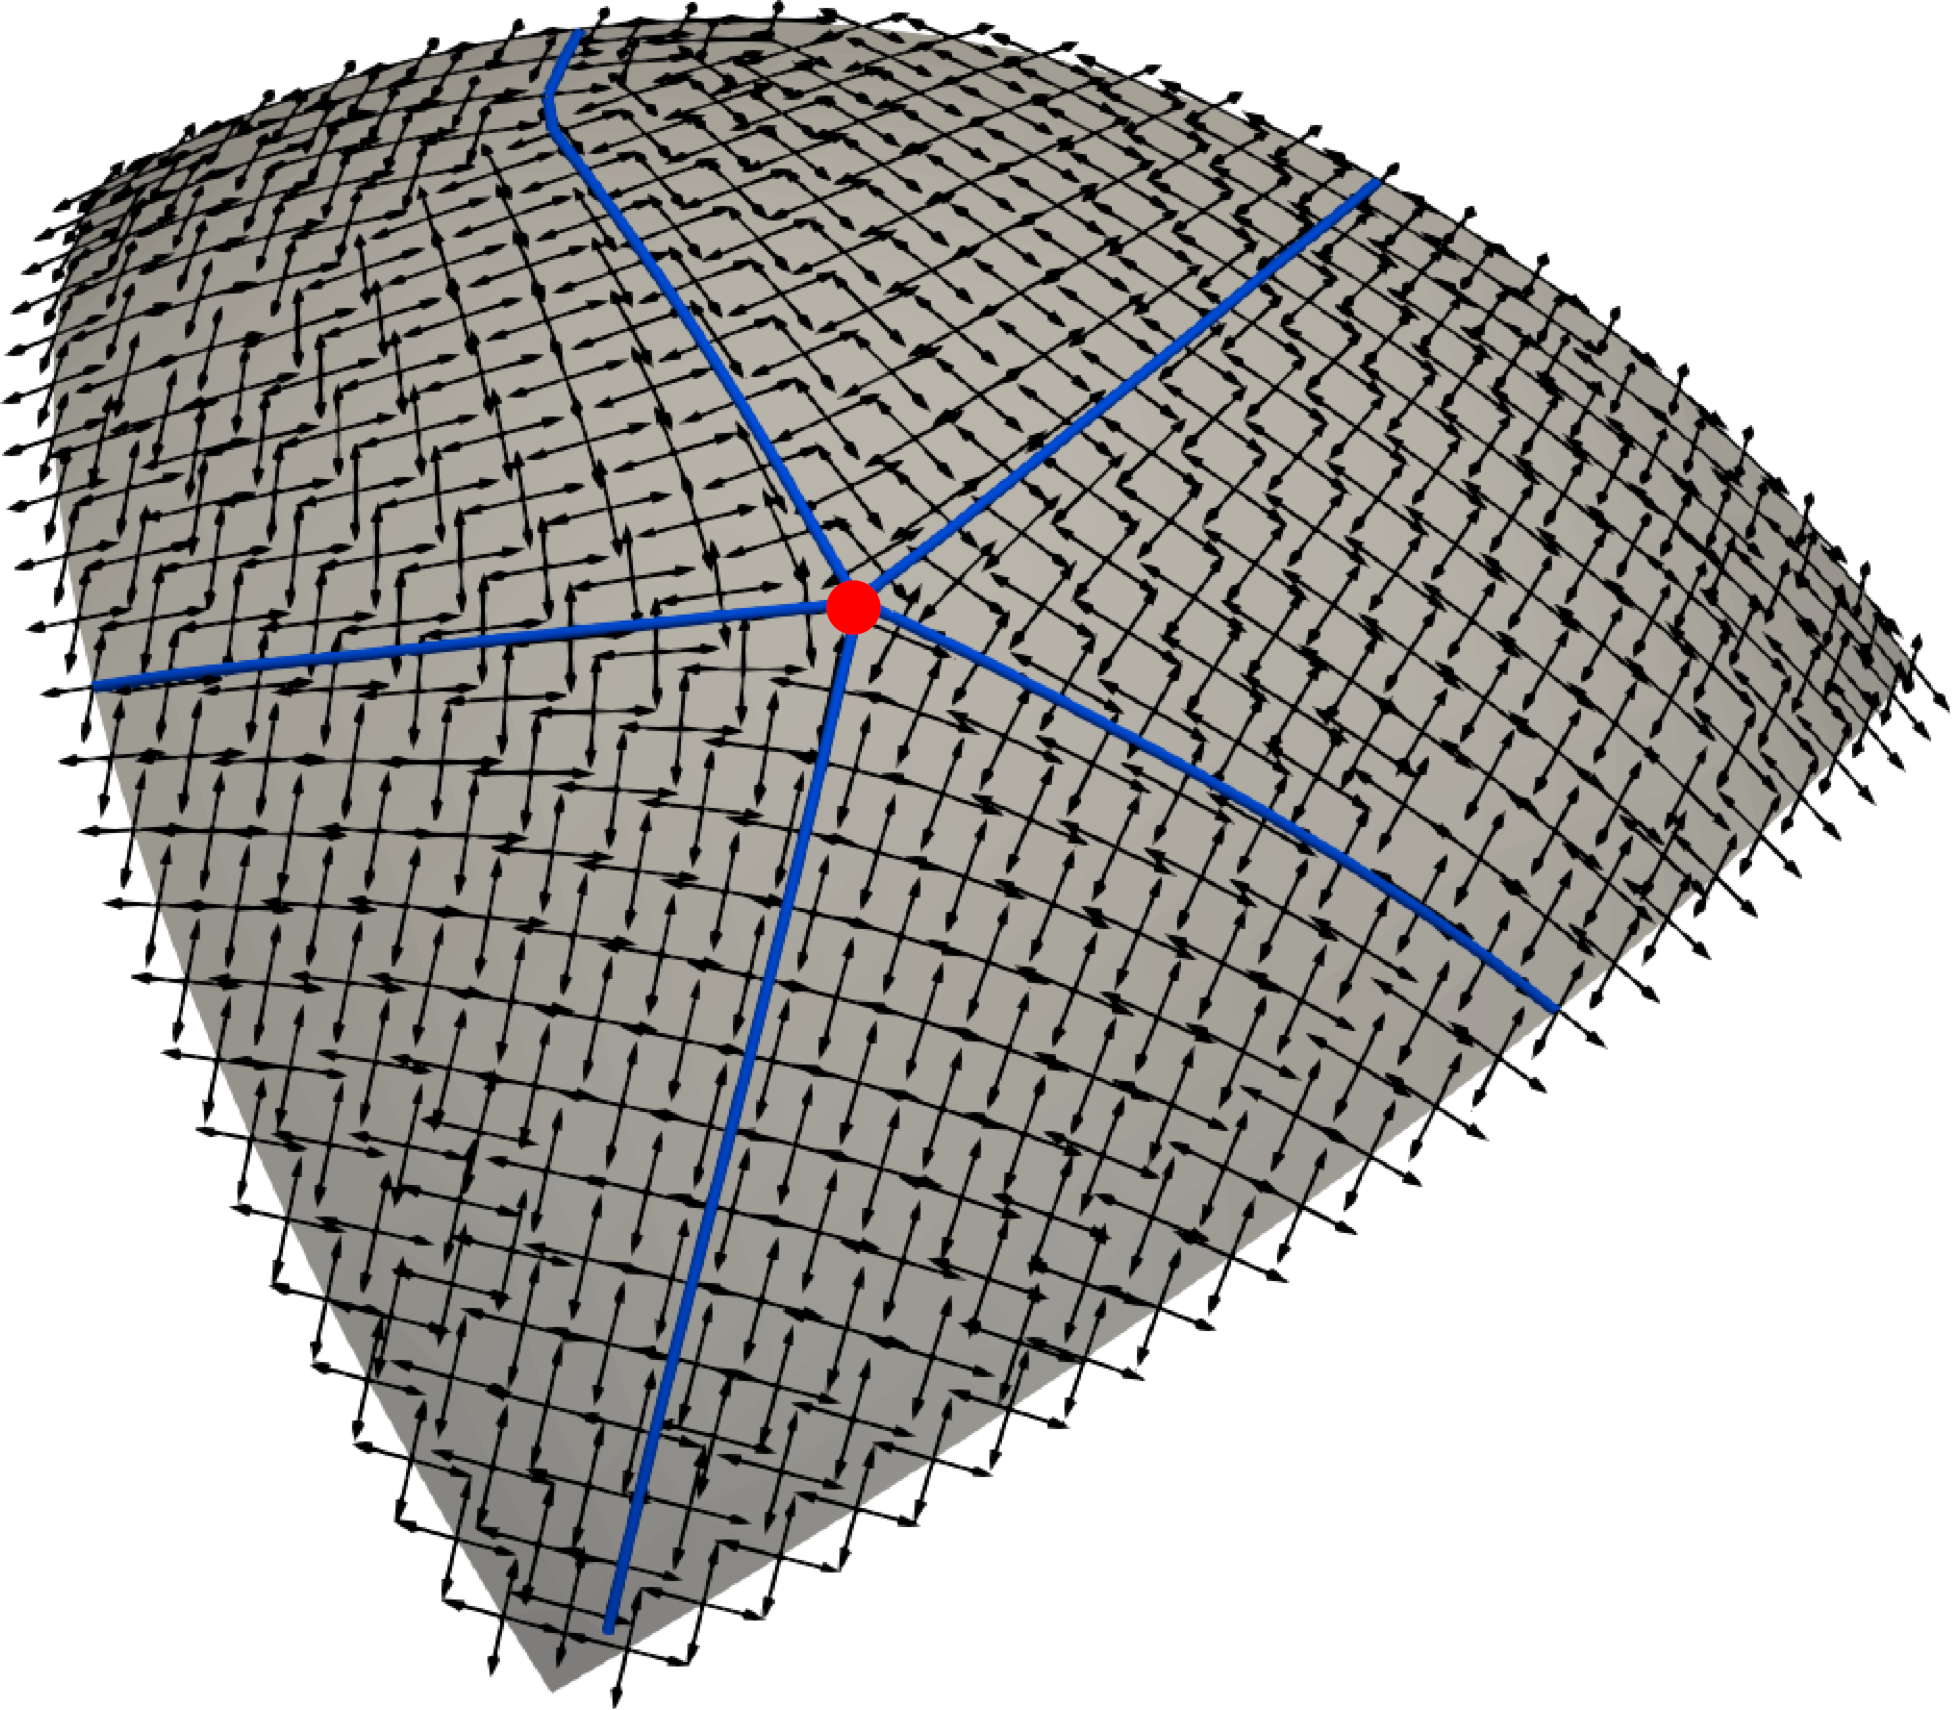
\includegraphics[scale=0.25]{images/surface_sepa_5.pdf}
\\[0.5cm]
  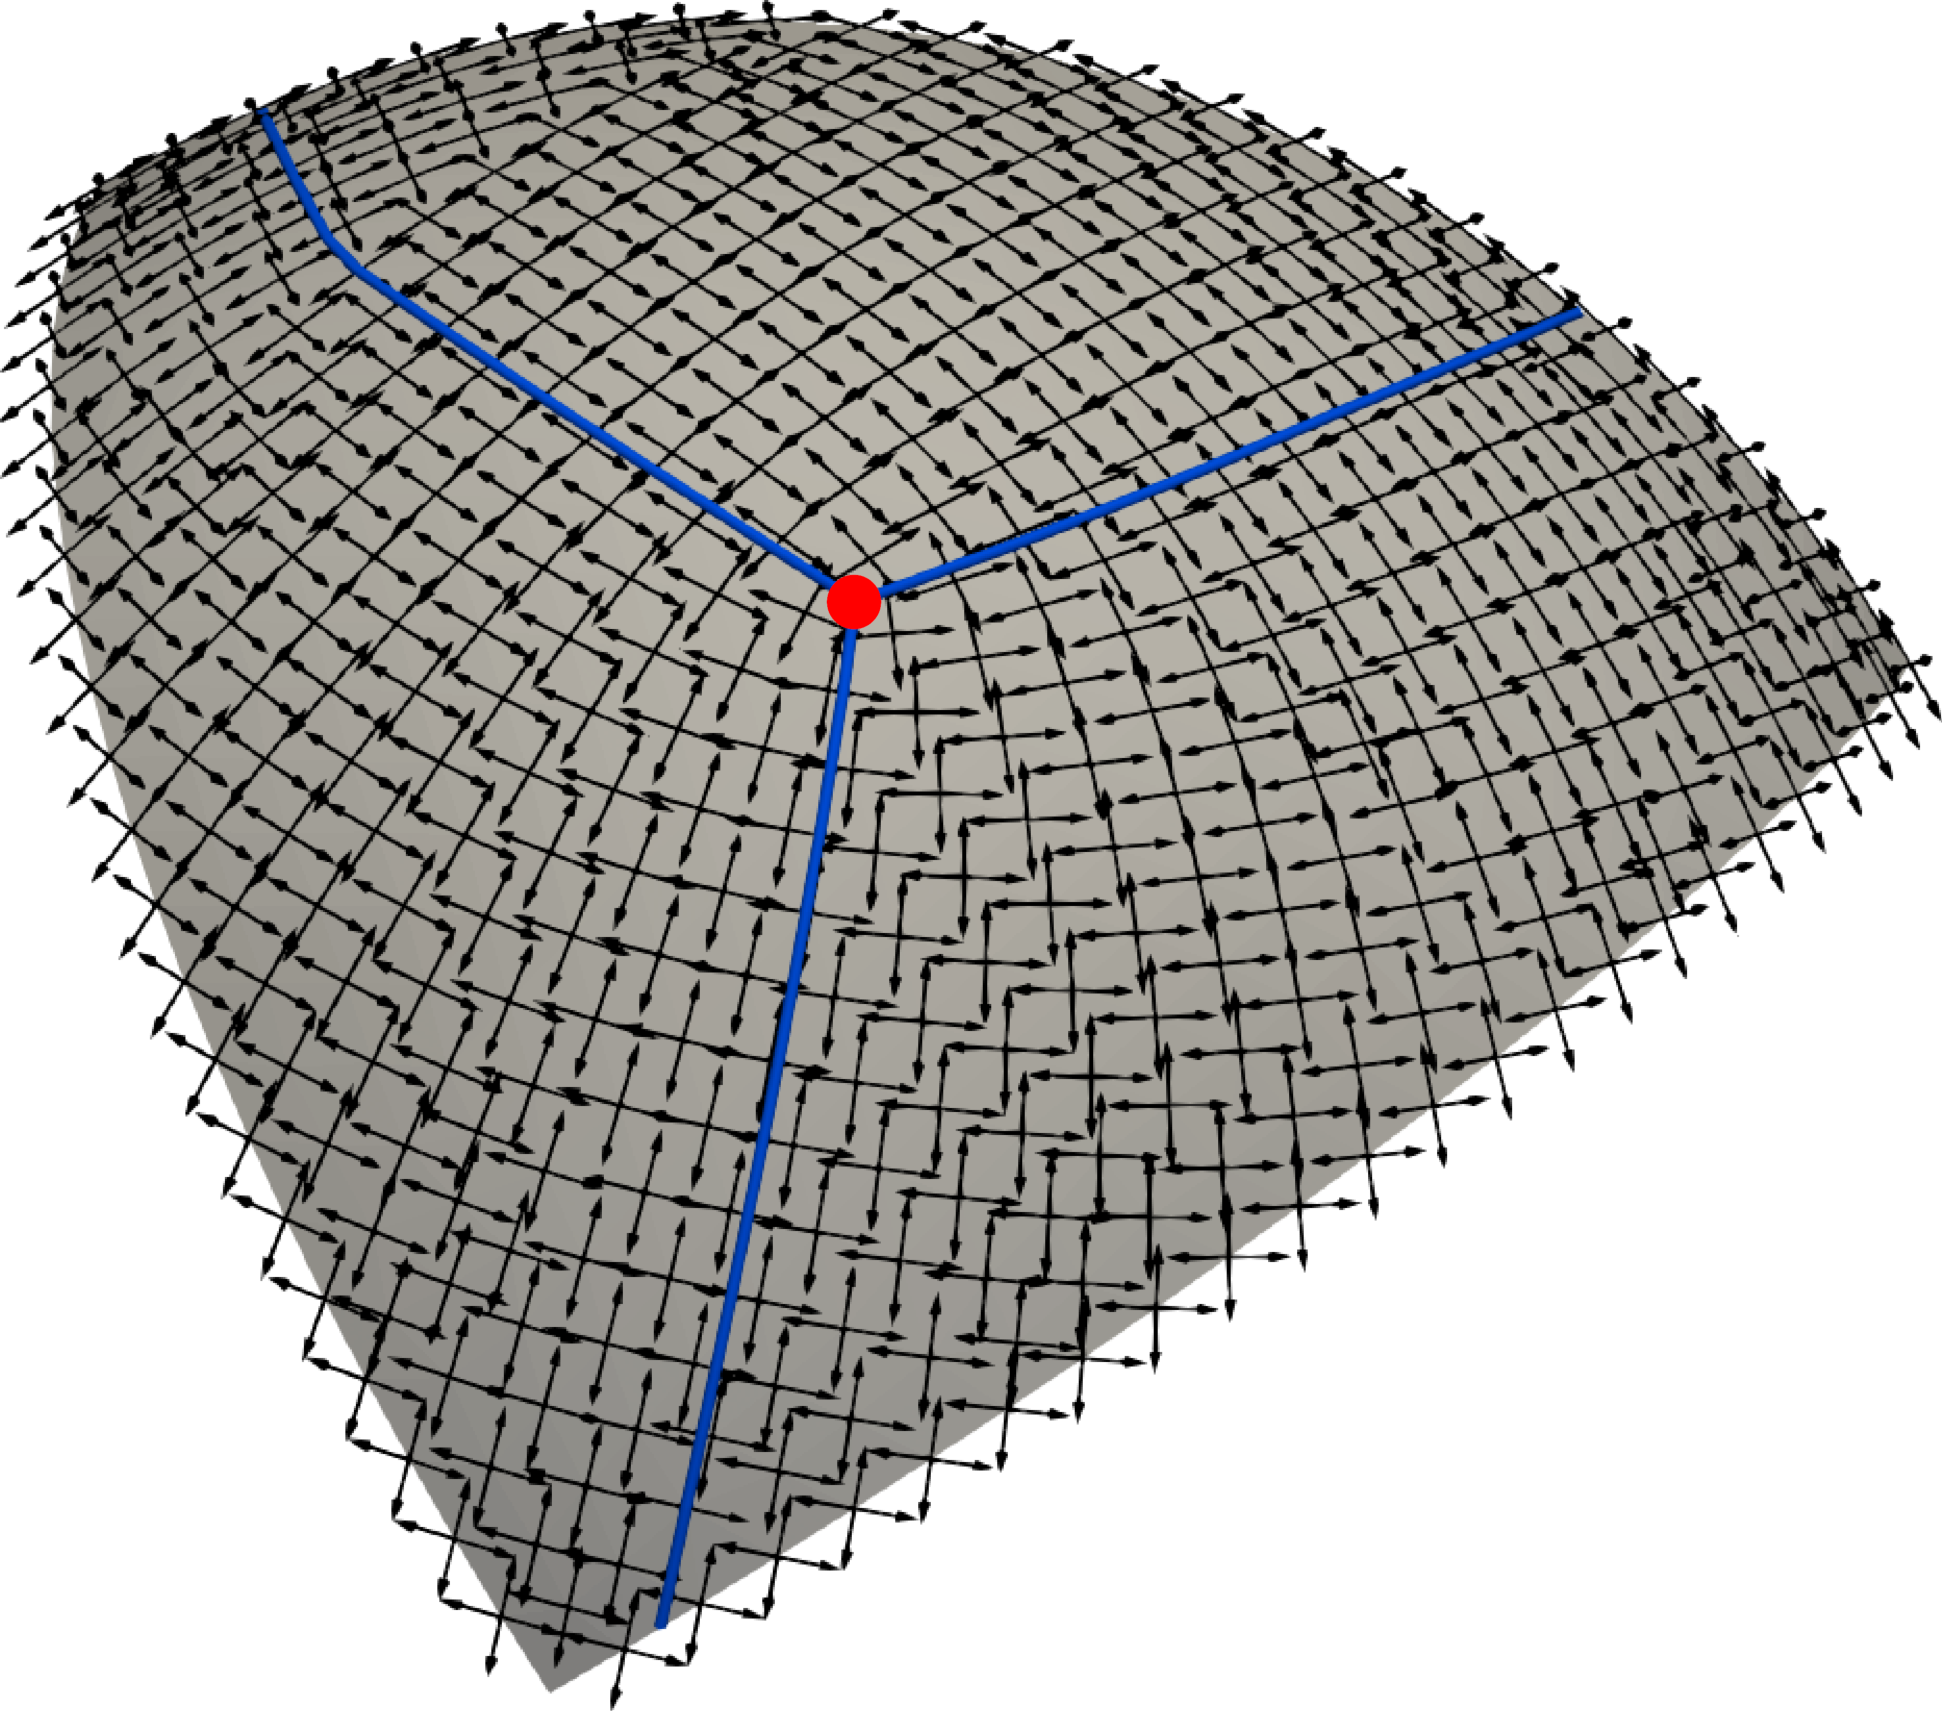
\includegraphics[scale=0.25]{images/surface_sepa_3.pdf}
  \caption{Gauche: Illustration des séparatrices émanant de points singuliers d'indice $-1/4$ (en haut) et d'indice $1/4$ (en bas).}
  \label{fig:separatrice_illustration_surface}
\end{figure}


Examinons maintenant ce que deviennent ces concepts dans un cadre discret. Soit $\Omega_h$ un maillage triangulaire de $\Omega$ vérifiant les contraintes définis dans la sous-section \ref{subsec:mesh_tri}. Nous reconstruisons la normale surfacique en chaque sommet de $\Omega_h$ en prenant une somme vectorielle des normales des triangles adjacents au sommet en question pondérées par l'aire des triangles. Soit $s$ un sommet de $\Omega_h$. La normale reconstruite en $s$ est donné par:
\begin{equation}
N(s)=\displaystyle\frac{1}{\displaystyle\sum_{T\in T_s}|T|}\left(\displaystyle\sum_{T\in T_s}|T|N_T\right),
\end{equation}
où $N_T$ désigne la normale au plan contenant le triangle $T$ et $T_s$ représente l'ensemble des triangles adjacents à $s$.

Nous abordons à présent la représentation $\bar{u}_h$ sur $\Omega_h$ d'un champ de croix presque-$\mathcal{C}^1$ $\bar{u}$ défini sur $\Omega$. On suppose que des valeurs nodales de $\bar{u}$ sont attribuées aux sommets du domaine $\Omega_h$. L'évaluation des écarts d'angle de la définition d'un triangle singulier \ref{def:triangle_singulier} s'effectue en projetant les croix associé aux sommets du triangle dans l'espace tangent du triangle. Ainsi la croix $\bar{u}(s)$ où $s$ est un sommet du triangle devient:
\begin{equation}
Proj(\bar{u}(s), N_T)=
\left\{
\begin{array}{ll}
\displaystyle\left\{c-(c.N_T).N_T,~ c\in\bar{u}(s)\right\} &\mbox{ si }\bar{u}(s)\neq 0,\\\\
0& \text{ sinon},
\end{array}
\right.
\end{equation}

Ensuite, nous définissons les zones singulières comme précédemment (voir la sous-section \ref{subsec:discr_champ_de_croix}), avec la contrainte supplémentaire qu'une zone singulière est réduite soit à un triangle unique, soit à deux triangles adjacents, soit aux triangles adjacents à un sommet où la valeur nodale du champ s'annule. En pratique, il sera nécessaire d'ajuster un maillage qui ne respecte pas ces contraintes. Étant donné que les points singuliers du champ croisé $\bar{u}$ sont isolés, il est toujours possible de respecter ces contraintes en affinant localement le maillage ou en effectuant des modifications (par exemple, via des opérations de retournement d'arêtes) sur un maillage qui ne les satisfait pas. La représentation $\bar{u}_h$ de $u$ est alors donnée par morceau sur chaque triangle $T$ par :\\

\begin{itemize}
\item[$\bullet$] pour tout $T\in\mathcal{T}_h$, $\bar{u}_h(s)$, où $s$ est un sommet de $T$ est égale à $0$ si $\bar{u}(s)=0$ sinon $\bar{u}_h(s)$ correspond à la projection de $\bar{u}(s)$ dans le plan tangent du triangle $T$.\\%[-0.3cm]

\item[$\bullet$] si $T\subset\Omega_h\backslash\mathbf{Z}$ alors pour tout $p\in T$, on pose:
$$
\left\{
\begin{array}{l}
\theta_1 = \theta_{\bar{u}_h}(s_1)\\\\
\theta_2 = \theta_1 + \delta\theta(\bar{u}_h(s_1),\bar{u}_h(s_2))\\\\
\theta_3 = \theta_2 + \delta\theta(\bar{u}_h(s_2),\bar{u}_h(s_3))
\end{array}
\right.
$$
où $s_1$, $s_2$ et $s_3$ sont les sommets du triangle $T$. La croix $\bar{u}_h(p)$ est alors donnée par:
$$
\left\{
\begin{array}{l}
\bar{u}_h(p)=\displaystyle\left\{\mathbf{R}_{N_T,\theta_p+m\frac{\pi}{2}}(X_T), ~m\in\mathbb{Z}\right\},\\\\
\theta_p=\displaystyle\sum_{i\in\llbracket1, 3\rrbracket}\lambda_i\theta_i,
\end{array}
\right.
$$
avec $(\lambda_i)_{i\in\llbracket 1, 3\rrbracket}$ les coordonnées barycentriques de $p$ dans le triangle $T$, $N_T$ la normale au plan contenant le triangle $T$ et $X_T$ le vecteur de référence arbitrairement choisi dans cet espace tangent. Autrement dit, ils vérifient $p=\sum_{i=1}^3\lambda_i s_i$ et $\sum_{i=1}^3\lambda_i=1$.\\
\item[$\bullet$] si $T\subset\mathbf{Z}$ et que pour tout sommet $s$ de $T$ on a $\bar{u}(s)\neq 0$ on commence par interpoler l'angle du champ de le champ de croix  le long des arêtes de $T$. On a alors pour tout $p\in T$:
\begin{itemize}
 \item si $p=S_Z$, alors $\bar{u}_h(p)=0$.\\
 \item sinon la croix $\bar{u}_h(p)$ est donnée par:
\begin{equation}
\label{eqn:etoilage_space}
\left\{
\begin{array}{l}
\bar{u}_h(p)=\bar{u}_h(\widetilde{p}),\\\\
\{\widetilde{p}\}=[S_Zp)\cap\partial Z.
\end{array}
\right.
\end{equation}
\end{itemize}
\item[$\bullet$] Sinon, si $T\subset\mathbf{Z}$, alors par construction, il existe un unique sommet $s$ de $T$ tel que $\bar{u}_h(s)=0$. On interpole alors l'angle du champ de croix sur l'arête de $T$ opposée à $s$. Ensuite, pour tout point $p$ appartenant à $T$, on utilise l'équation \eqref{eqn:etoilage_space} pour calculer $\bar{u}_h(p)$.
\end{itemize}


\section{Partitionnement de $\partial\Omega_h$ et maillage}
%\label{sec:partitionnement_omega_h}

Nous abordons maintenant la question du partitionnement du maillage $\Omega_h$ représentant le domaine $\Omega_h$. De façon similare à ce que nous avons présenté dans le cas planaire, nous nous basons sur l'algorithme \ref{alg:discr_algo_main}.

Les points singuliers coïncidant exactement avec les points $S_Z$ où $Z\subset\mathbf{Z}$ leur recherche consiste donc à retrouver ces points. Il faut ensuite déterminer le nombre de séparatrices par points singuliers ainsi que leurs directions de départ grâce à la fonction $W_{p_0}^\gamma$ où ici $p_0$ désigne le point singulier et $\gamma$ est une paramétrisation du bord $\partial Z_{p_0}$ de la zone singuliere $Z_{p_0}$ contenant $p_0$. On intègre ensuite les lignes de champs sur la surface triangulée. Cependant, contrairement au cas planaire les triangles ne se trouvant pas tous dans le même plan. Le passage d'une ligne de champ d'un triangle à son voisin se fait alors en projetant le vecteur d'intégration dans le plan du triangle voisin grâce à la formule de Rodrigues \cite{trucco1998introductory}. Nous illustrons cela sur la figure
\ref{fig:draw_sepa_space}.

\begin{figure}[h!]
\centering
\begin{subfigure}{0.65\textwidth}
    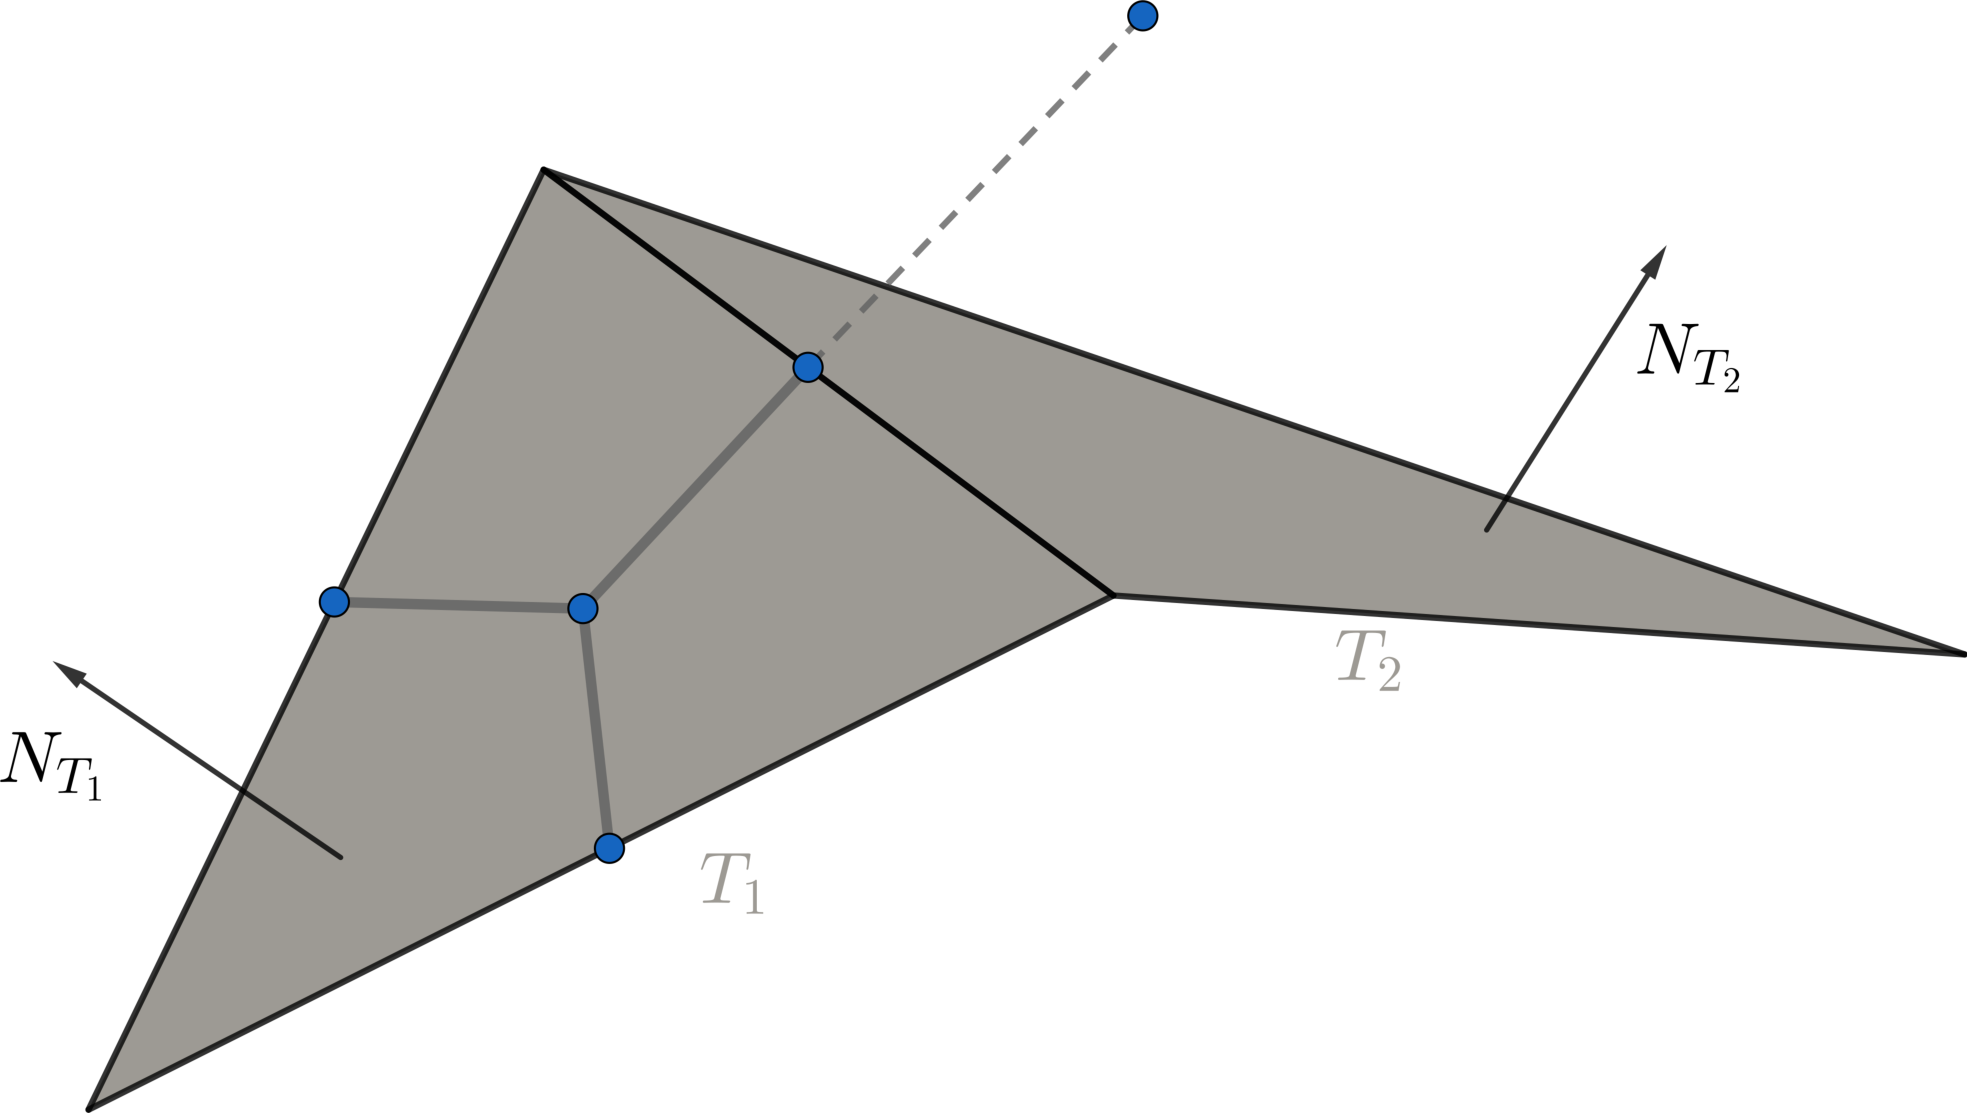
\includegraphics[width=\textwidth]{images/draw_sepa_space_1.pdf}
    %\caption{Champ scalaire $\phi_h$ (en randian)}
    %\label{fig:alignment_2}
\end{subfigure}
\\[0.5cm]
\begin{subfigure}{0.65\textwidth}
    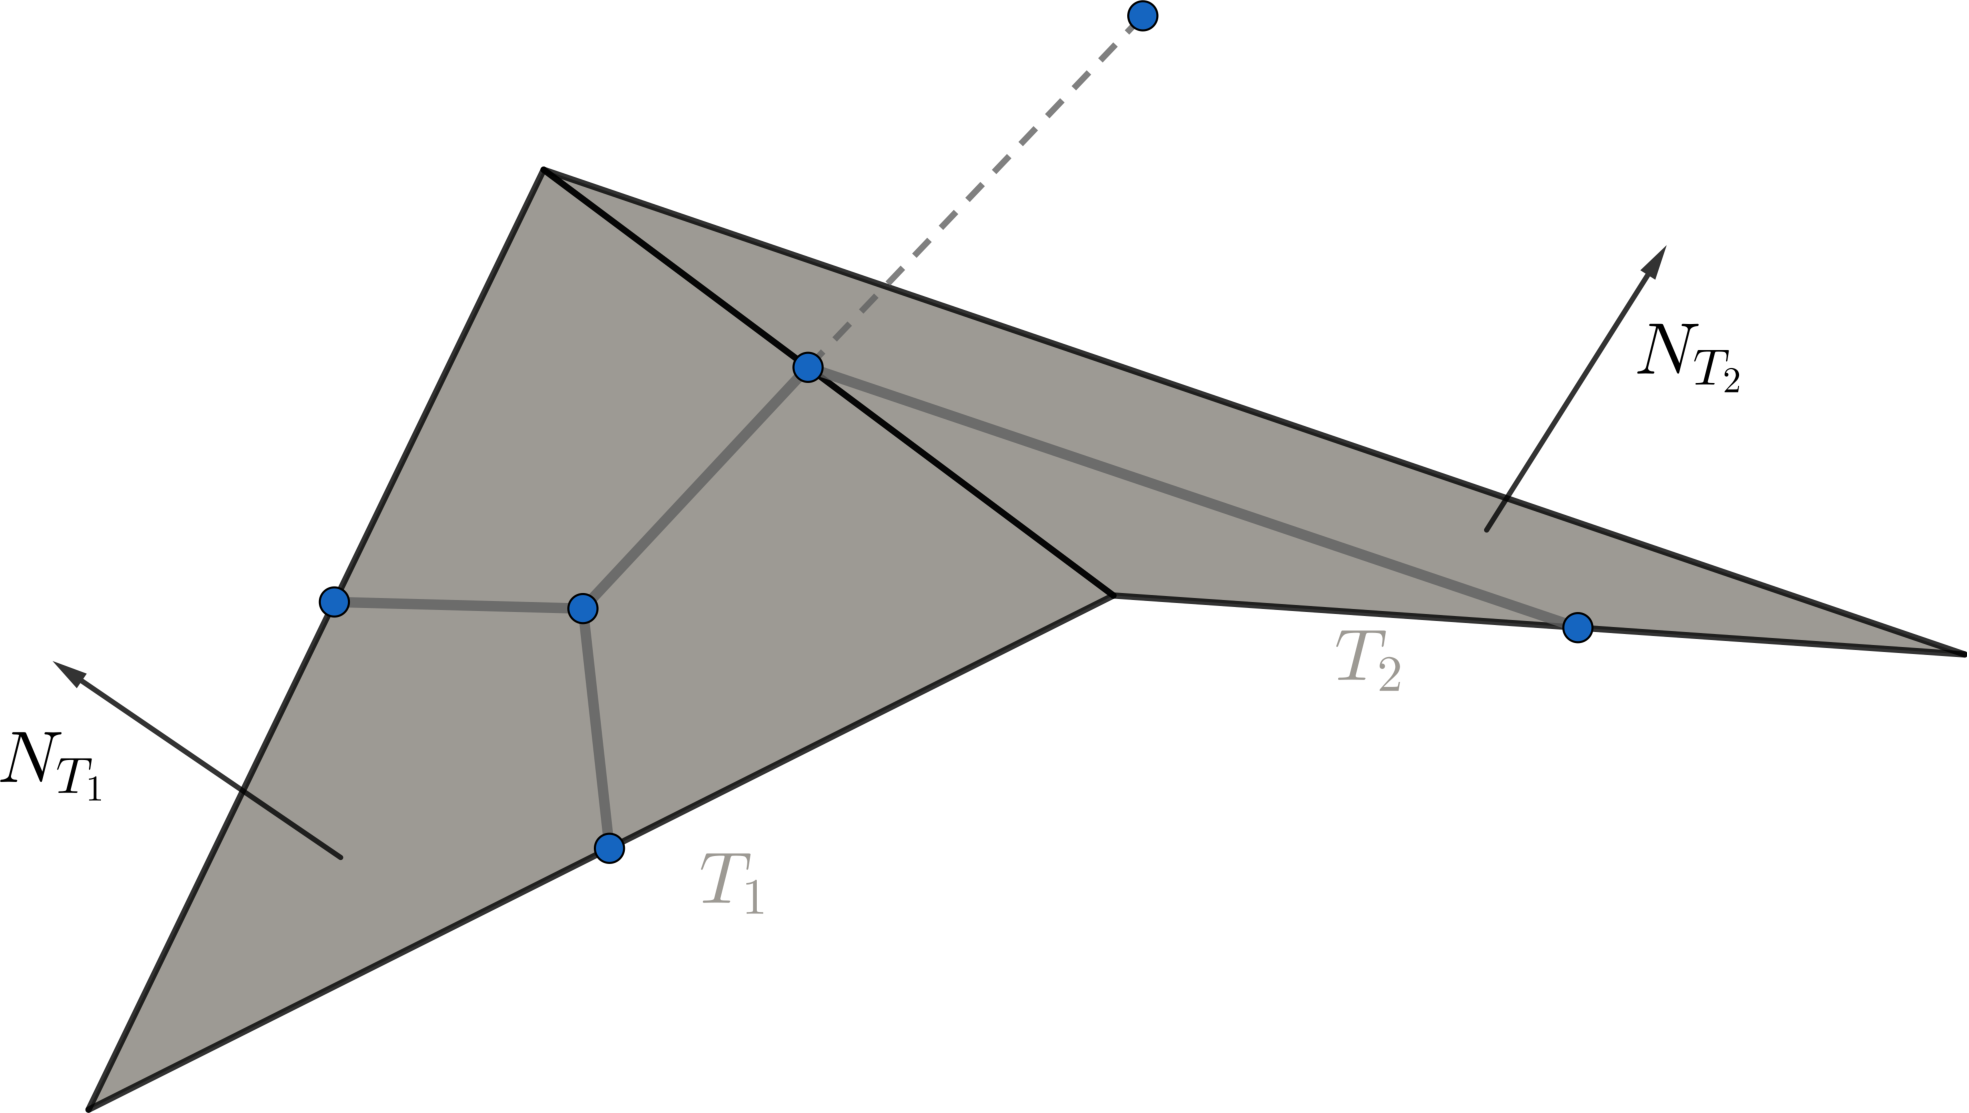
\includegraphics[width=\textwidth]{images/draw_sepa_space_2.pdf}
    %\caption{Maillage.}
    %\label{fig:alignment_4}
\end{subfigure}
\caption{Illustration du processus d'intégration d'une ligne de champ.}
\label{fig:draw_sepa_space}
\end{figure}

La traversée d'un triangle singulier (voir figure \ref{fig:singulier_sepa_space})  reste équivalente à ce qui a été présenté dans le chapitre \ref{chap:alorithme} de même que la fusion de séparatrices. Nous illustrons cela sur la figure \ref{fig:draw_sepa_space}.

\begin{figure}[!h]
  \centering
  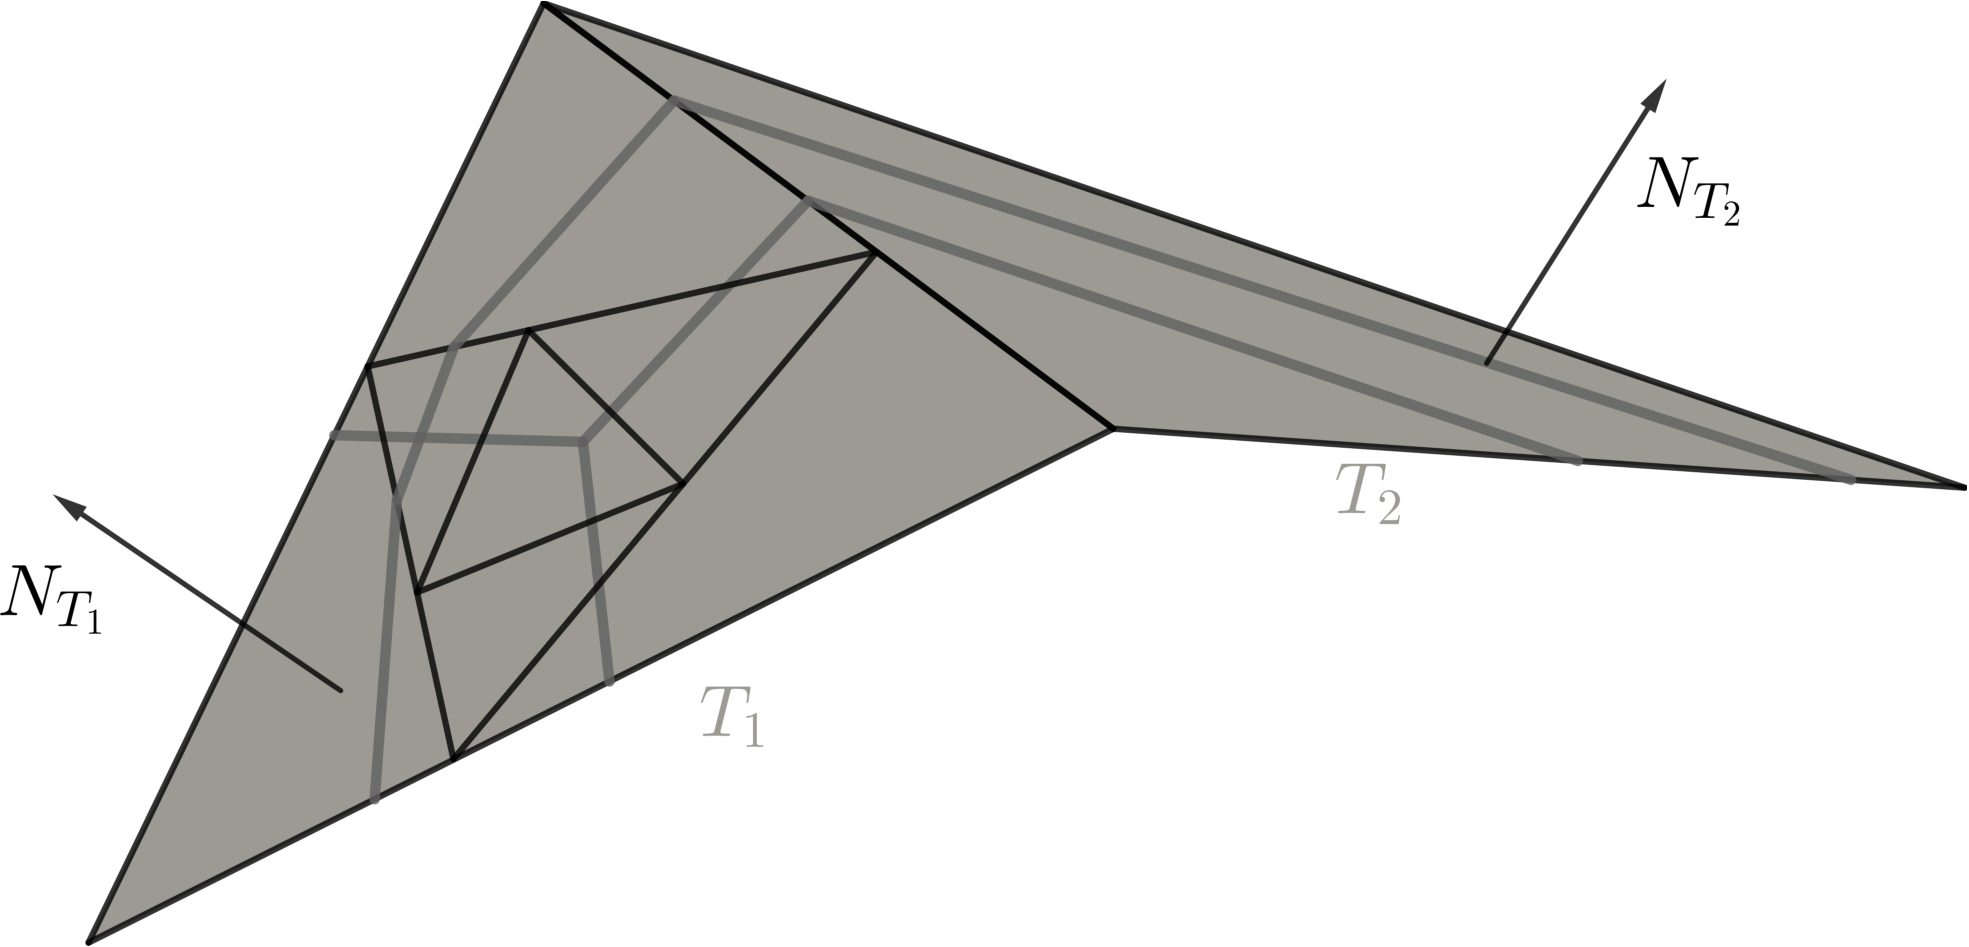
\includegraphics[scale=0.32]{images/singulier_sepa_space.pdf}
  \caption{Illustration de la traversé par une séparatrice d'un triangle singulier.}
  \label{fig:singulier_sepa_space}
\end{figure}

Les séparatrices du champ de croix sont construites simultanément en incrémentant chacune d'elles progressivement, et le processus de fusion est réalisé tel que décrit dans le chapitre \ref{chap:alorithme}. Un illustration en est donnée sur la figure \ref{fig:fusion_space}.


\begin{figure}[h!]
\centering
\begin{subfigure}{0.525\textwidth}
    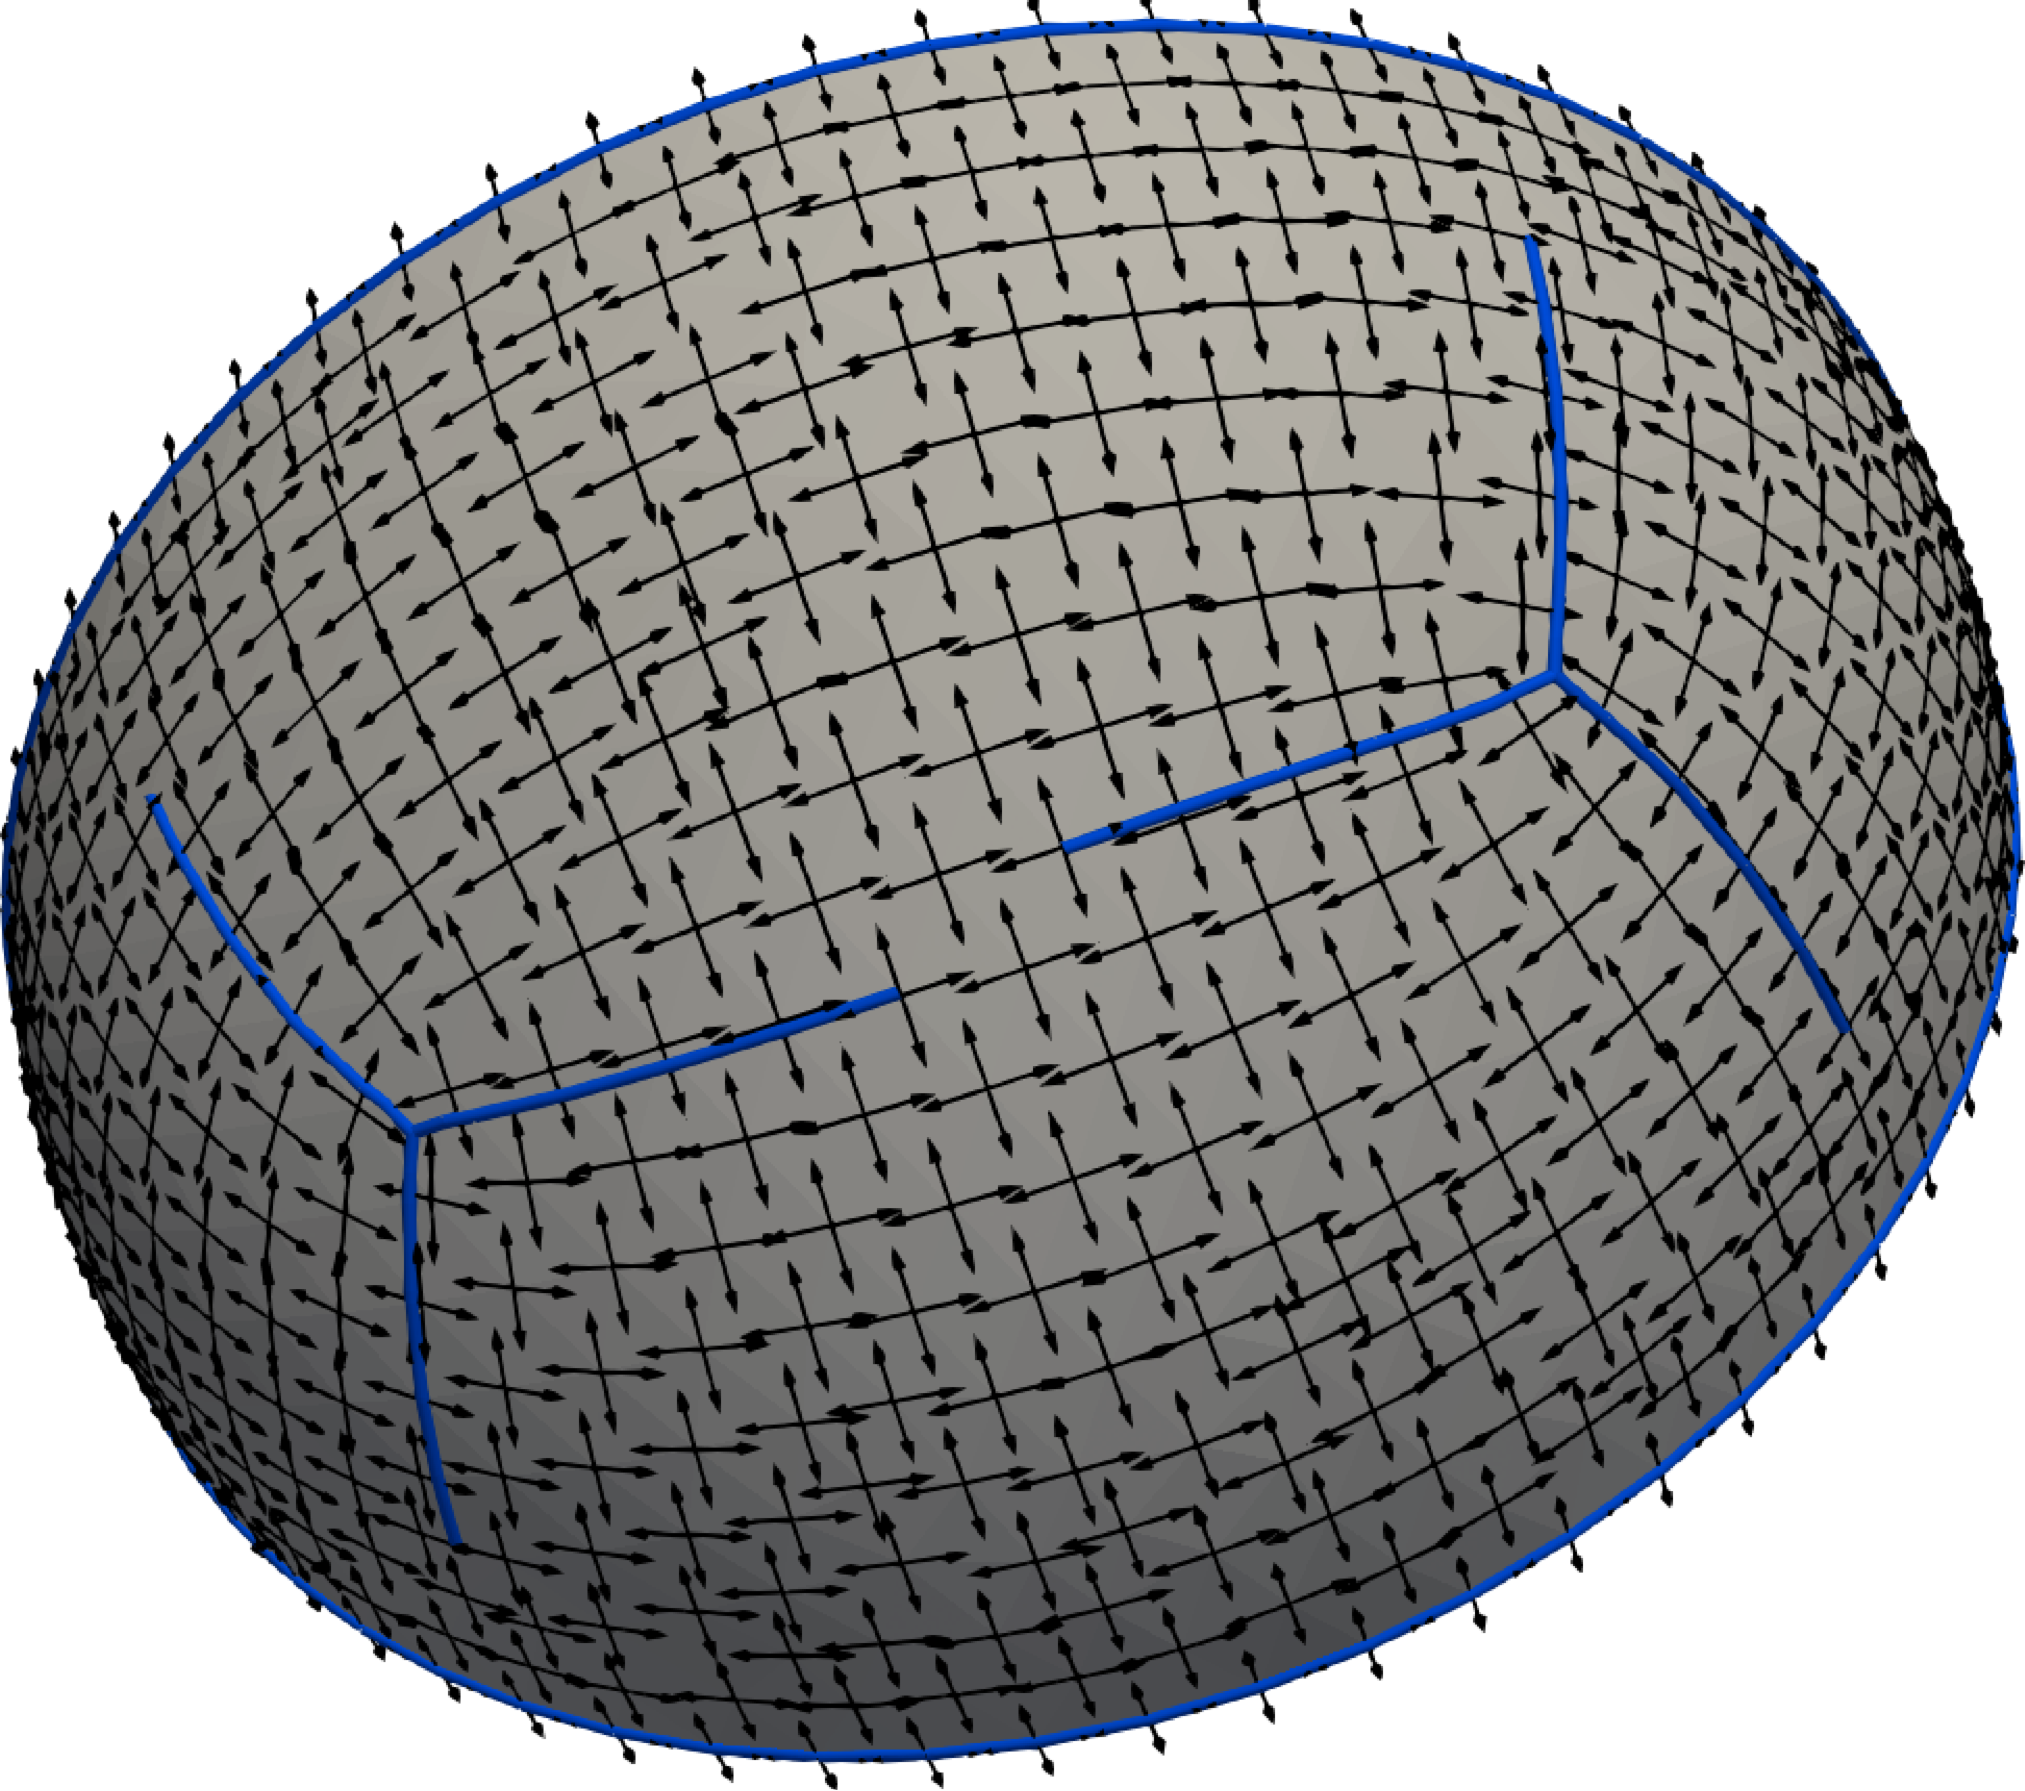
\includegraphics[width=\textwidth]{images/detect_fusion_space.pdf}
    \caption{Détection d'une fusion.}
    %\label{fig:alignment_2}
\end{subfigure}
\\[0.2cm]
\begin{subfigure}{0.525\textwidth}
    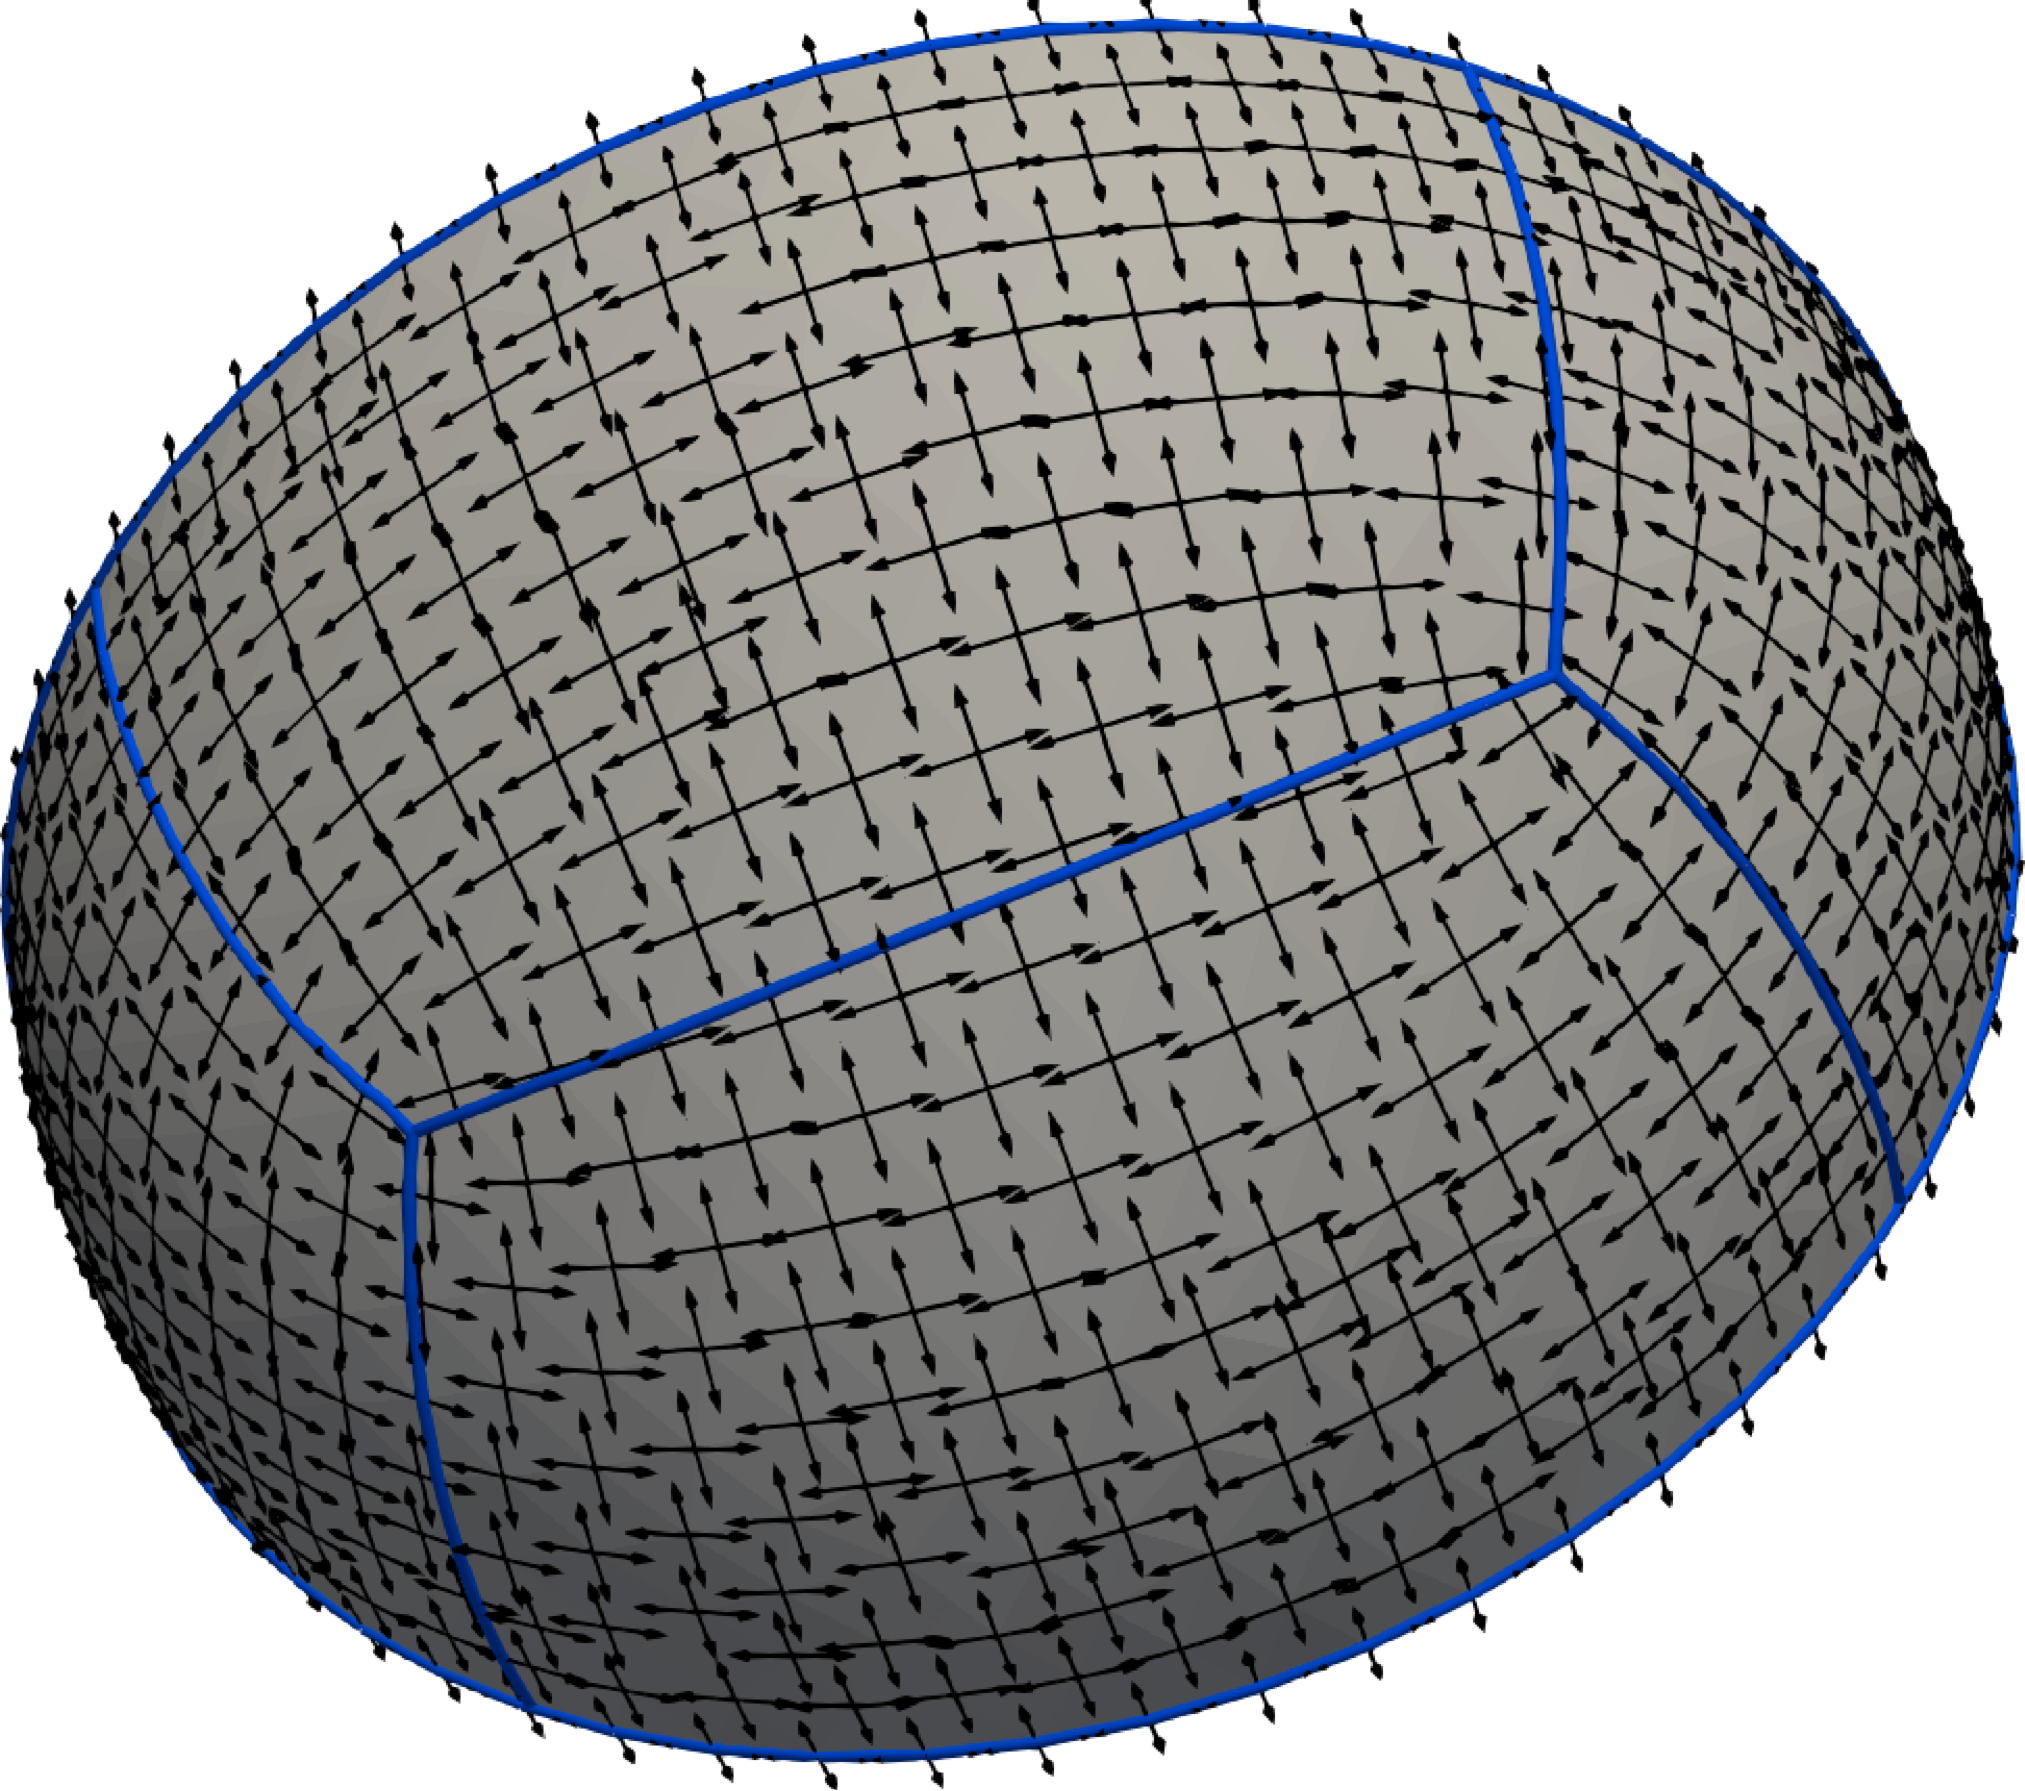
\includegraphics[width=\textwidth]{images/fusion_space.pdf}
    \caption{Fusion.}
    %\label{fig:alignment_4}
\end{subfigure}
\caption{Illustration de la fusion de deux séparatrices.}
\label{fig:fusion_space}
\end{figure}

Les figure \ref{fig:intersection_space} et \ref{fig:extraction} montrent les étapes d'assemblage à savoir l'intersection de separatrices et l'extraction des partitions en tant que sous- maillage.

\begin{figure}[!h]
  \centering
  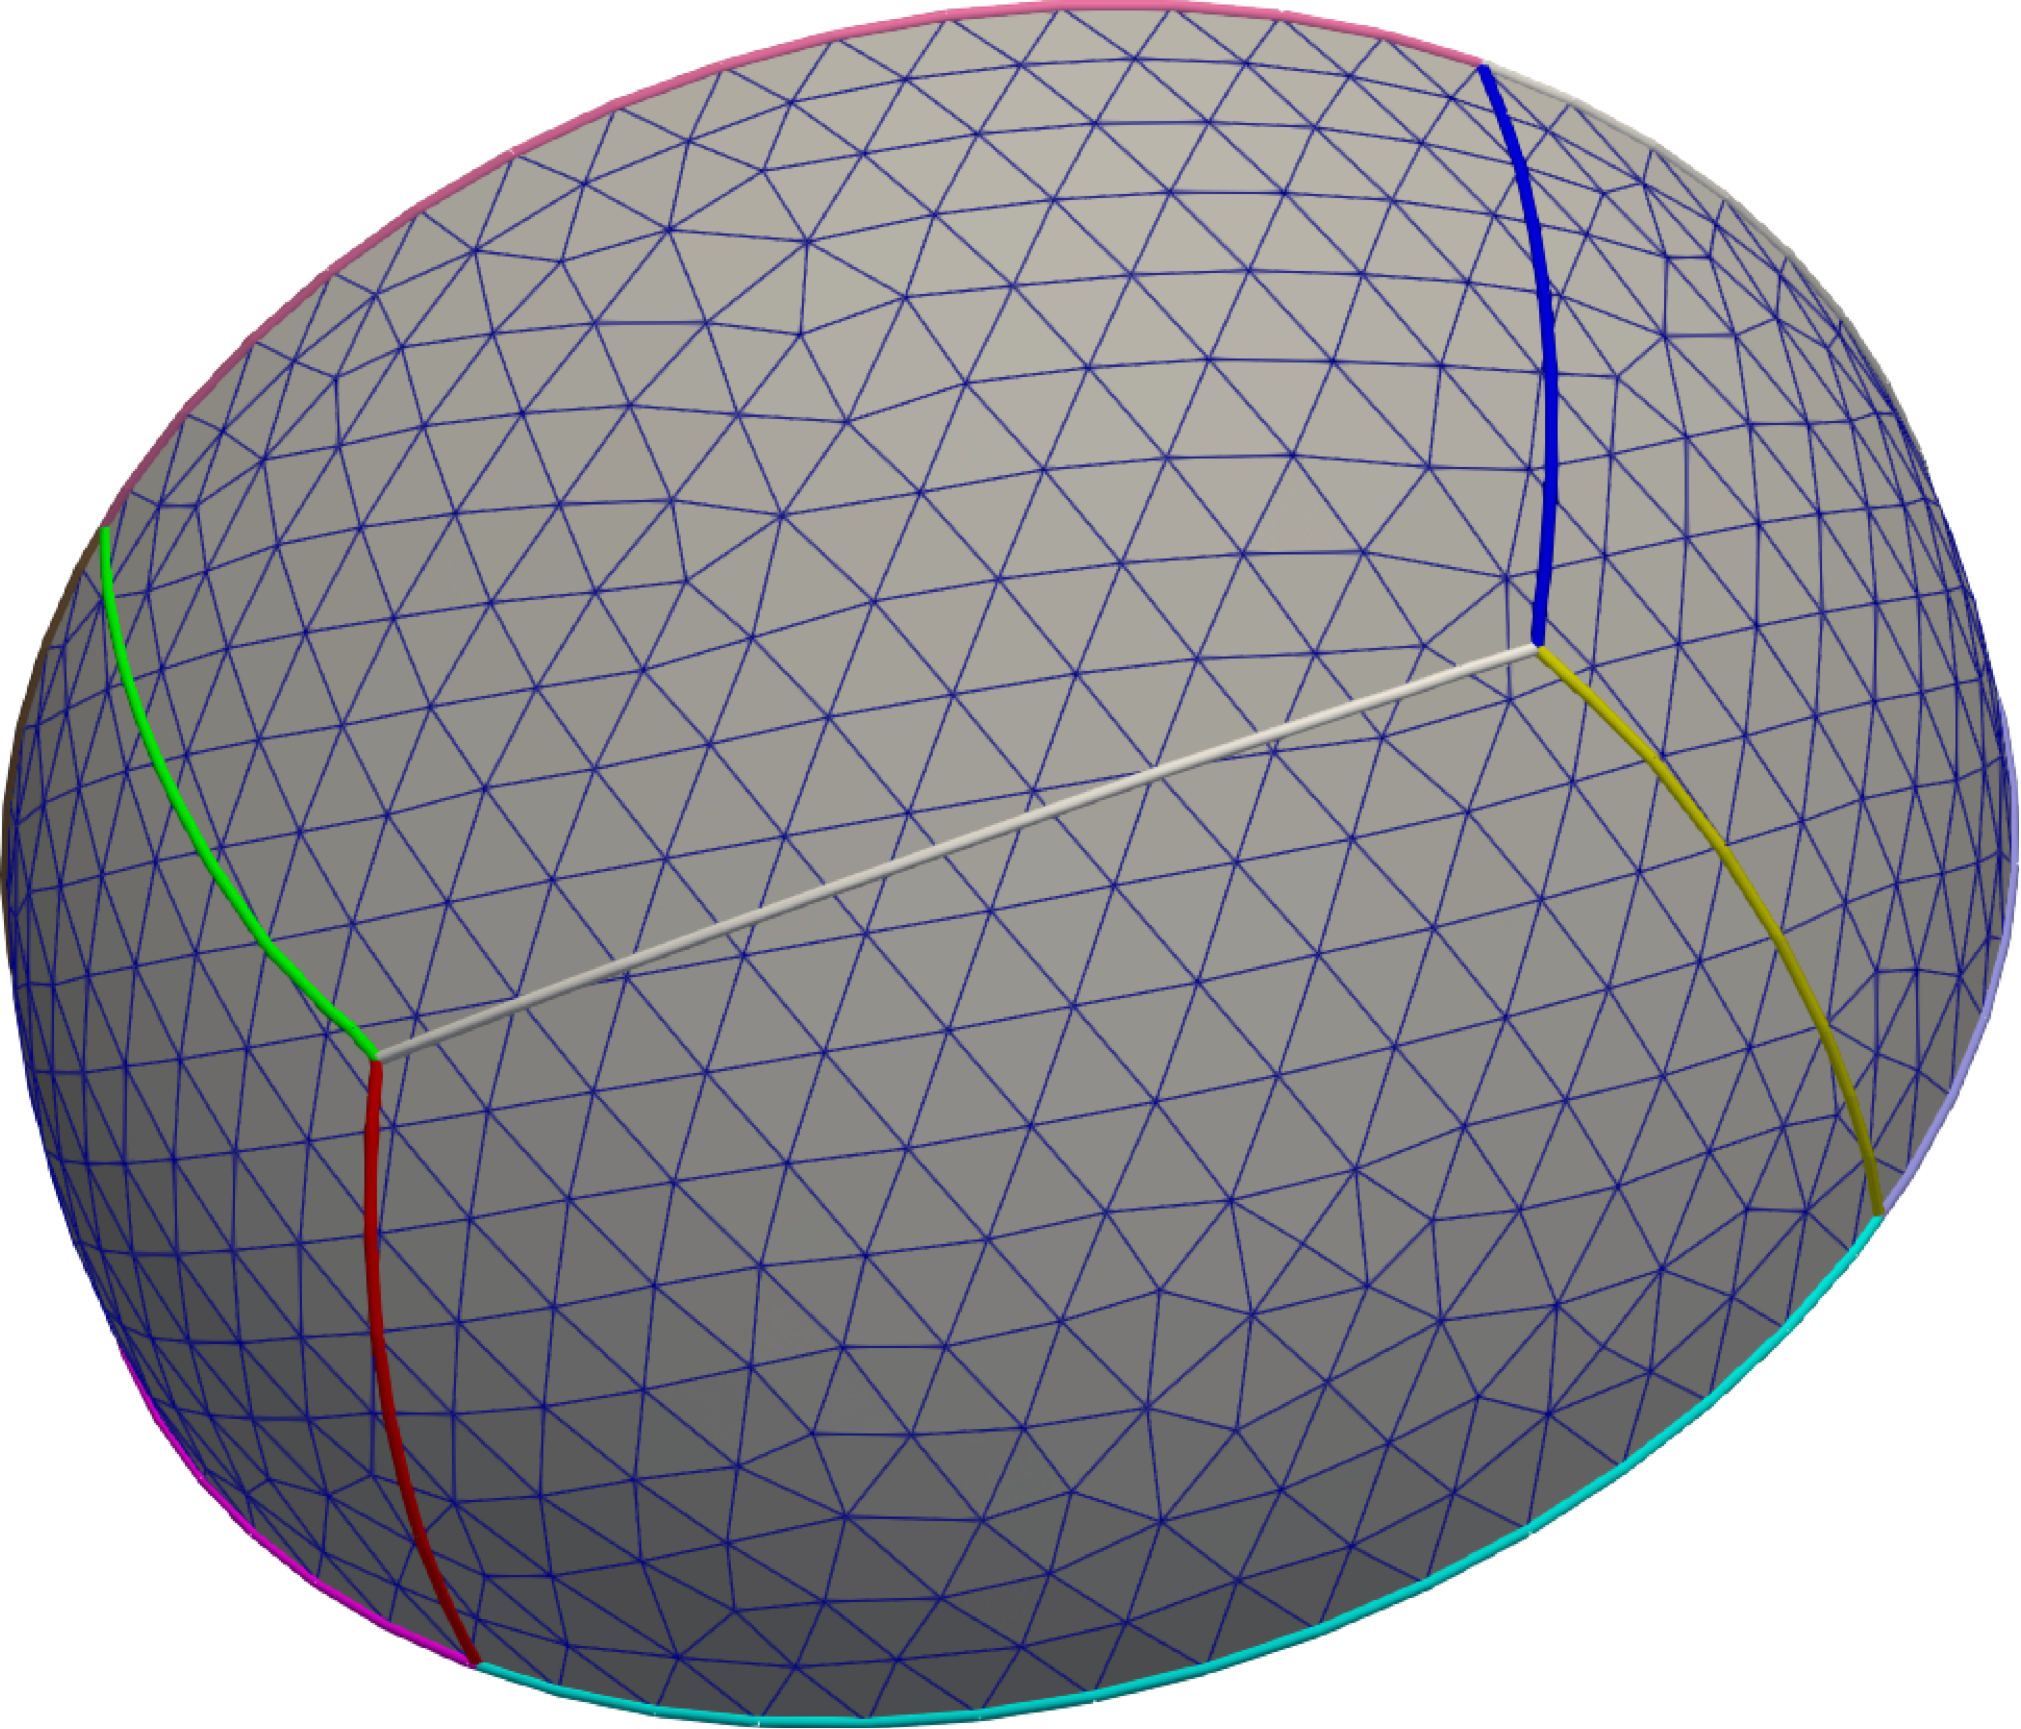
\includegraphics[scale=0.235]{images/intersection_space.pdf}
  \caption{Illustration de l'intersection de séparatrices.}
  \label{fig:intersection_space}
\end{figure}

\begin{figure}[h!]
\centering
\begin{subfigure}{0.49\textwidth}
    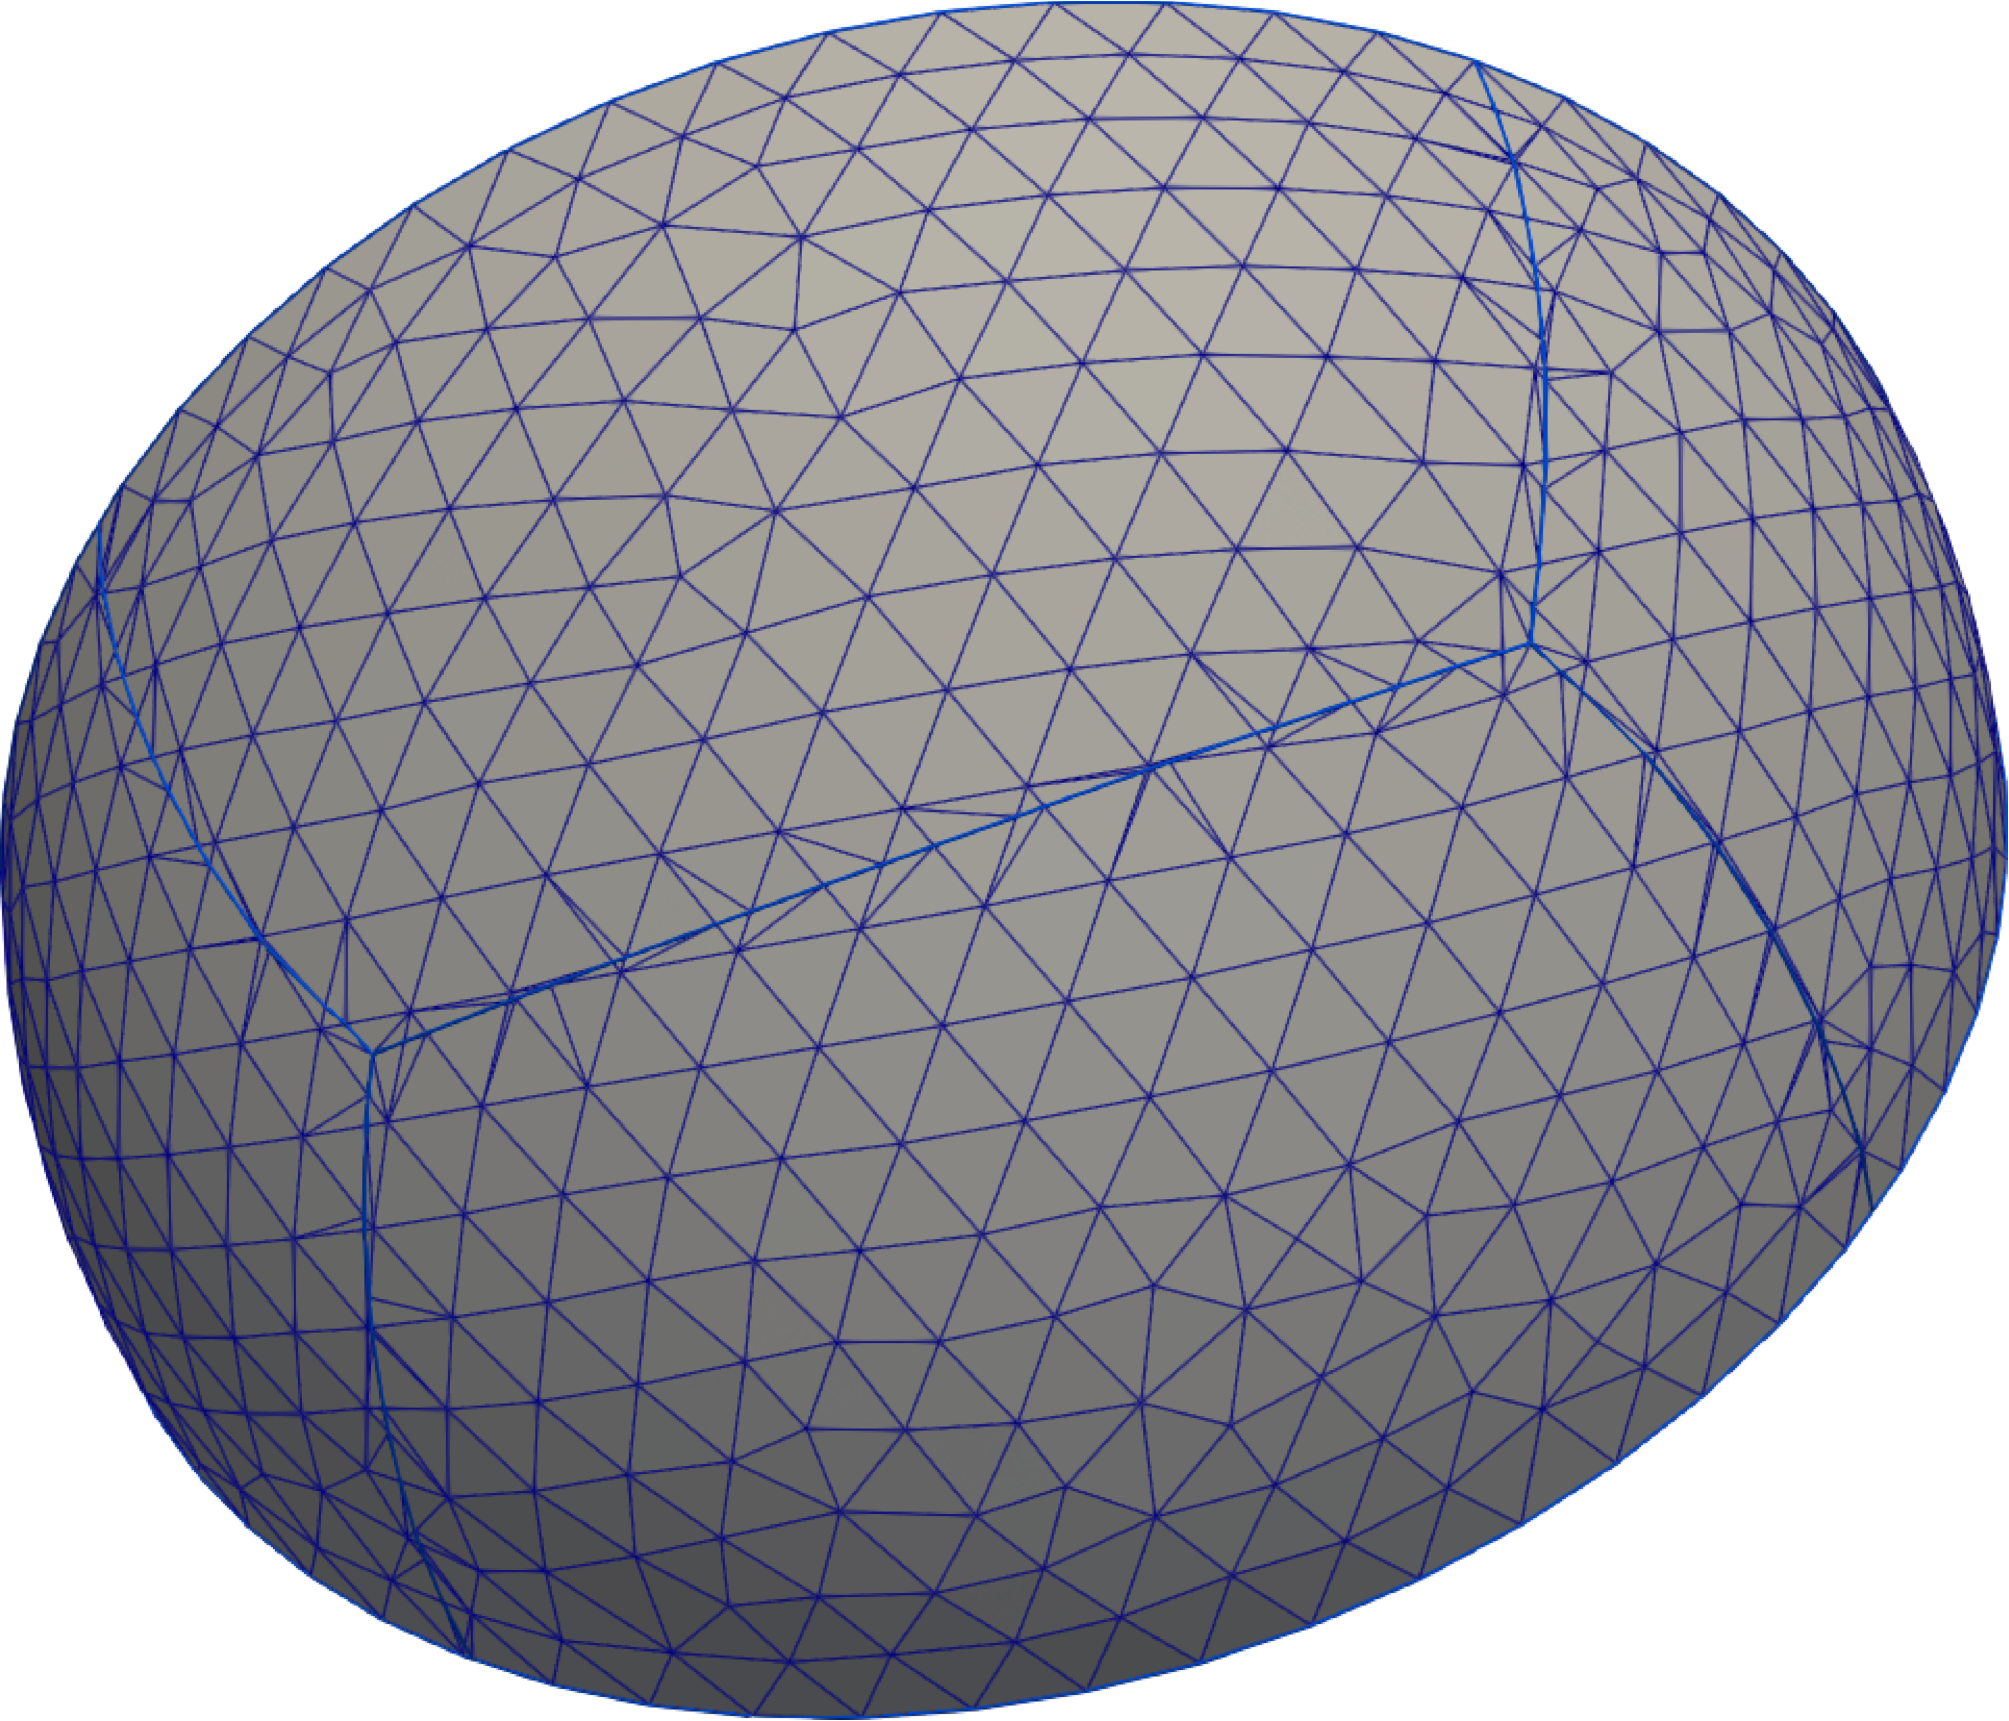
\includegraphics[width=\textwidth]{images/split_triangles_space.pdf}
    %\caption{Champ scalaire $\phi_h$ (en randian)}
    %\label{fig:alignment_2}
\end{subfigure}
\hfill
\begin{subfigure}{0.49\textwidth}
    \includegraphics[width=\textwidth]{images/eclatement_space.pdf}
    %\caption{Maillage.}
    %\label{fig:alignment_4}
\end{subfigure}
\caption{Extraction des séparatrices en tant que sous-maillage.}
\label{fig:extraction}
\end{figure}

Lorsque toutes les partitions obtenues comportent quatre côtés, nous générons ensuite le maillage quadrilatéral pour chaque partition en utilisant la méthode exposée dans la sous-section \ref{method_based_edp}. Nous en fournissons une illustration dans la figure \ref{fig:quad_space}.

\begin{figure}[!h]
  \centering
  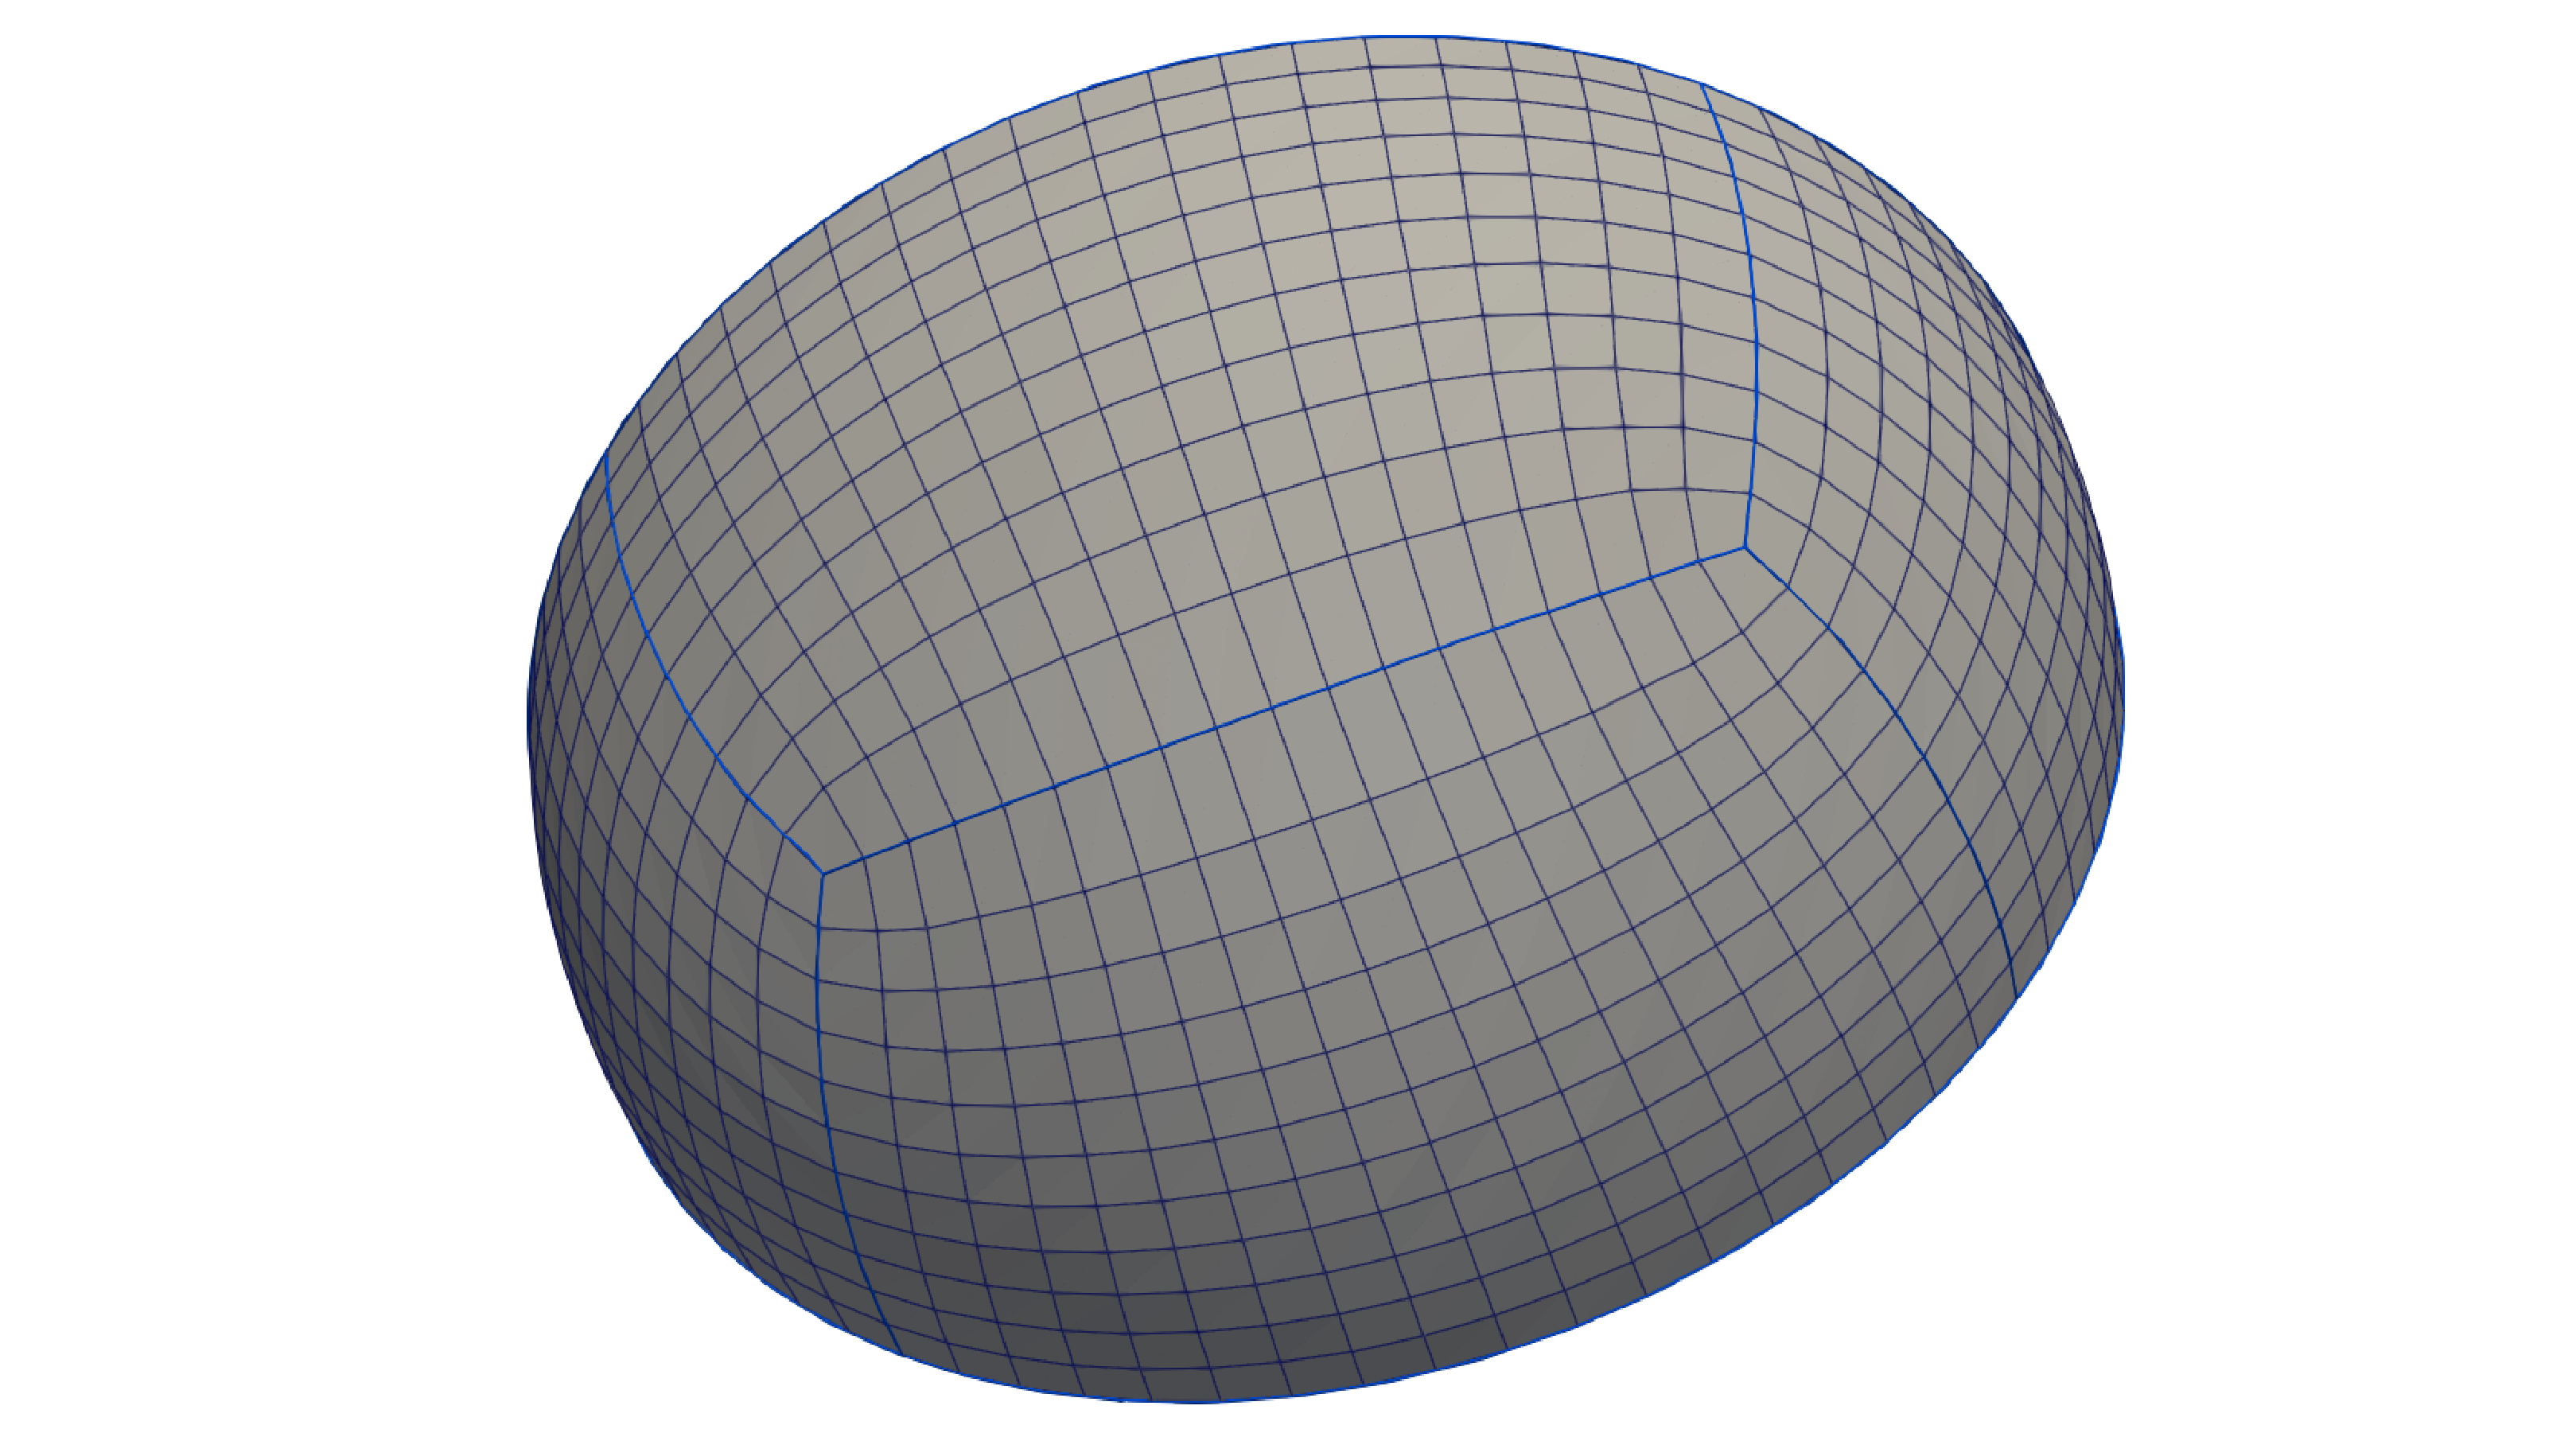
\includegraphics[scale=0.24]{images/quad_space.pdf}
  \caption{Maillage de chaque partition.}
  \label{fig:quad_space}
\end{figure}

\section{Extension des résultats principaux du cas planaire}

Le théorème ci-dessous énonce les conditions nécessaires à l'utilisation d'un champ de croix spécifié pour subdiviser une surface courbe dans l'espace en régions caractérisées par quatre côtés.

\begin{theorem}
\label{thm:theorem1_space}
Considérons $\bar{u}$ comme un champ de croix presque-$\mathcal{C}^1$ défini sur $\Omega$, aligné avec $\partial\Omega$, tel que $0 < \text{Card}(\mathcal{S}_{\bar{u}}) < \infty$. Pour tout point $p \in \Omega$, supposons que $id_{\bar{u}}(p) = k/4$, où $k \in \mathbb{Z}$ et $k \leq 1$. Si l'algorithme de partitionnement \ref{alg:algo_main}, appliqué à $\bar{u}$, converge et que chaque région $\mathcal{R}$ du partitionnement satisfait $\chi(\mathcal{R})=1$, alors le partitionnement résultant constitue une décomposition de $\Omega$ en régions à quatre côtés.
\end{theorem}

La démonstration de ce théorème suit la même logique que celle du théorème \ref{thm:theorem1}. Cependant, il est important de noter l'introduction d'une hypothèse supplémentaire concernant les régions issues du partitionnement. Cette condition spécifie qu'une région $\mathcal{R}$ résultant du partitionnement doit satisfaire l'équation $\chi(\mathcal{R})=1$. Dans le contexte planaire, cette contrainte était toujours satisfaite. Cependant, dans l'espace, pour des surfaces de genre non nul, aucune garantie préalable n'est donnée quant à la nullité du genre des partitions créées. Ainsi, l'expression $\chi(\mathcal{R}) = 2 - 2g - b$ n'est pas toujours égale à $1$, où $g$ et $b$ représentent respectivement le genre et le nombre de composantes connexes du bord de $\mathcal{R}$ (voir figure \ref{fig:double_tore}).

\begin{figure}[!h]
  \centering
  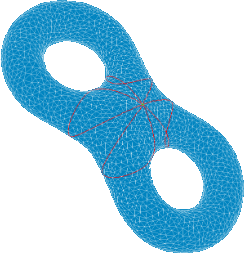
\includegraphics[scale=0.8]{images/double_tore.png}
  \caption{Partitionnement d'un double tore à partir d'un point singulier d'indice $-2$: source \cite{chen2018metric}.}
  \label{fig:double_tore}
\end{figure}

Une approche pour résoudre ce problème pourrait consister à introduire des points supplémentaires permettant de générer de nouvelles séparatrices dans la partition concernée. Cela pourrait conduire, par une subdivision successive, à la création de nouvelles séparatrices de genre plus faible, jusqu'à ce que l'on obtienne finalement des partitions de genre nul.



\paragraph{\'Etude de l'opération d'alignement}

Considérons maintenant que $\Omega$ est simplement connexe et que le champ de croix $\bar{u}$ n'est pas nécessairement aligné sur $\partial\Omega$ mais vérifie:
\begin{itemize}
 \item[$\bullet$] $0\leq Card(\mathcal{S}_{\bar{u}})Card(\mathcal{B})<\infty$,\\
 \item[$\bullet$] Pour tout point $p\in\mathcal{S}_{\bar{u}}$, $id_{\bar{u}}(p)=k/4$, avec $k\in\mathbb{Z}$ et $k\leq 1$,\\
 \item[$\bullet$] Etant donné $I_p$ définit pour tout $p$ par:
\begin{equation}
I_p=\displaystyle\frac{k}{4}\mbox{ avec }k\in\mathbb{Z}\mbox{ et }k\leq 1
\end{equation}
on a:
 \begin{equation}
    \label{eqn:principe_hypothese_u_space}
    \sum_{p\in(\Omega\backslash\partial\Omega)\cap\mathcal{S}_{\bar{u}}}id_{\bar{u}}(p)=\chi(\Omega)-\sum_{p\in\mathcal{B}}I_p.
\end{equation}
où $\mathcal{B}$ désigne l'ensemble des points tel que $I_p\neq 0$.\\
\end{itemize}
L'opération d'alignement consiste alors à calculer le champ de croix $\bar{v}$ pour tout $p\in\Omega$ défini par:
\begin{equation}
\bar{v}(p)=
\left\{
\begin{array}{ll}
\mathbf{R}(\phi(p))\bar{u}(p) & \mbox{ si } p\in\Omega\backslash(\mathcal{B}\cup\mathcal{S}_{\bar{n}}\cup\mathcal{S}_{\bar{u}}),\\[0.5cm]
\bar{n}(p) & \mbox{ si } p\in(\mathcal{S}_{\bar{u}}\cap\partial\Omega)\backslash(\mathcal{B}\cup\mathcal{S}_{\bar{n}}),\\[0.5cm]
0 & \mbox{ si } p\in\mathcal{B}\cup\mathcal{S}_{\bar{n}}.
\end{array}
\right.
\label{eqn:principe_def_v_space}
\end{equation}
où $\phi:\Omega\longrightarrow\mathbb{R}$ est définie comme la solution de l'équation de Laplace suivante:
\begin{equation}
\left\{
\begin{array}{lcll}
\Delta\phi &=& 0 &\mbox{ dans }\Omega,\\[0.5cm]
\phi(\gamma(t))&=&\psi(t)-\displaystyle\sum_{s\in\gamma^{-1}(\mathcal{B}\cup\mathcal{S}_{\bar{n}})}2\pi I_{\gamma(s)}& \mbox{ sur } \gamma^{-1}(\partial\Omega\backslash(\mathcal{B}\cup\mathcal{S}_{\bar{n}}\cup\mathcal{S}_{\bar{u}})).
\end{array}
\right.
\label{eqn:principe_def_phi_space}
\end{equation}
Dans ce contexte, $\gamma$ représente une paramétrisation de la frontière $\partial\Omega$ sur l'intervalle $[0, 1]$ dans le sens positif par rapport à l'orientation de $\Omega$, et $\psi$ est le relèvement continu de l'angle $(\widehat{\bar{n}, \bar{u}})$ entre le champ de croix $\bar{n}$ et le champ de croix $\bar{u}$ le long de $\gamma$.

La formulation de la condition de bord de l'équation \ref{eqn:principe_def_phi_space} est motivée par l'absence de référence globale dans ce cas particulier (surface courbe dans l'espace). Une alternative consiste à construire un champ de croix sur $\Omega$ sans aucun point singulier et à le considérer comme une référence globale sur la surface. Nous avons adopter la méthode de la chaleur pour la diffusion, telle que présentée dans \cite{sharp2019vector}. Cette méthode propage un vecteur donné en fonction de l'équation de la chaleur, permettant ainsi la construction d'un cadre de référence global pour la surface. Cela facilite le calcul précis des angles du champ croisé et son alignement avec la frontière de la surface non-plane.

Plus précisément, nous construisons un champ de vecteurs $w$ sur la surface en utilisant l'équation \eqref{eqn:heatequation}, avec des conditions aux limites de Neumann homogènes. Nous amorçons la résolution en initialisant l'équation avec un champ de vecteurs égal à un vecteur arbitraire dans l'espace tangent d'un point arbitraire et mis à zéro partout ailleurs sur la surface. En résolvant cette équation sur une très courte période de temps, nous obtenons un champ de vecteurs dépourvu de singularités. L'étape suivante consiste à générer un repère en chaque point en effectuant une rotation du champ de vecteurs obtenu.

\begin{equation}
\left\{
\begin{array}{lcll}
\displaystyle\frac{\partial w}{\partial t} & = & \nabla^2 w &\mbox{ dans }\Omega,\\[0.5cm]
\nabla w.n&=&0 & \mbox{ sur } \partial\Omega.
\end{array}
\right.
\label{eqn:heatequation}
\end{equation}
où $n$ désigne la normale sortante au bord de $\Omega$. La Figure \ref{solutionheat} présente un exemple de la solution de l'équation, tandis que la Figure \ref{globalframe} illustre le repère global résultant obtenu. Nous exposons ensuite le processus d'alignement à partir d'un champ de croix non aligné avec le bord du domaine (voir Figure \ref{nonalign}). Ce champ de croix est ensuite aligné grâce au processus d'alignement, où les angles sont calculés à partir du champ de référence global. On obtient alors un découpage en régions à quatre côtés, comme présenté sur la Figure \ref{align}. D'autres illustrations sont présentées sur la Figure \ref{another}.

\begin{figure}[!h]
\centering
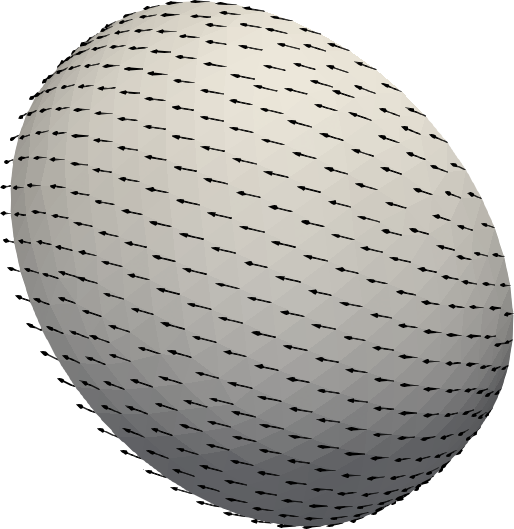
\includegraphics[scale=0.4]{images/vector.png}
\caption{Champ de vecteur obtenu par la méthode de diffusion de chaleur \cite{sharp2019vector}.}
\label{solutionheat}
\end{figure}

\begin{figure}[!h]
\centering
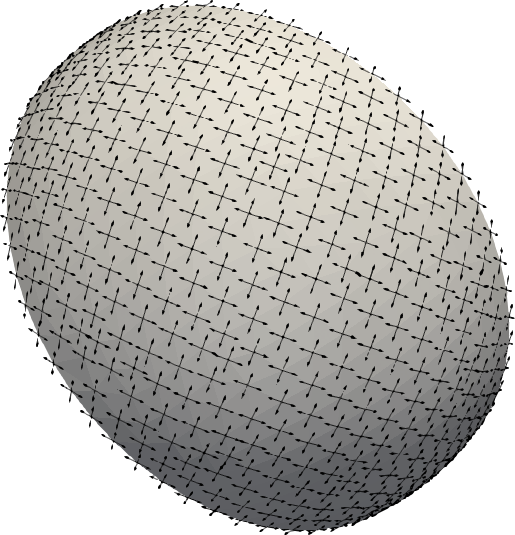
\includegraphics[scale=0.4]{images/frame.png}
\caption{Référence globale.}
\label{globalframe}
\end{figure}

\begin{figure}[!h]
\centering
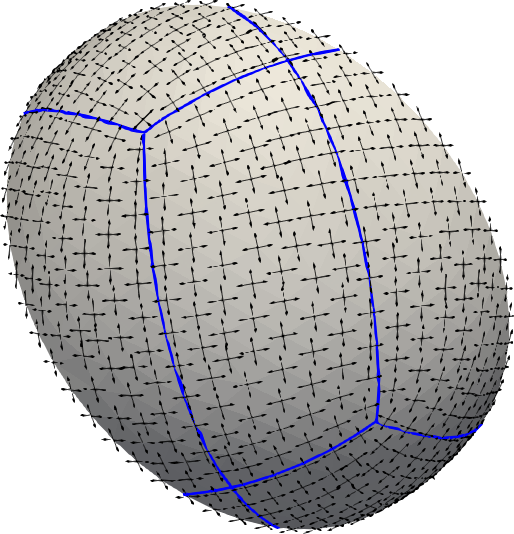
\includegraphics[scale=0.38]{images/nonalign.png}
\caption{Champ de croix non aligné.}
\label{nonalign}
\end{figure}


\begin{figure}[!h]
\centering
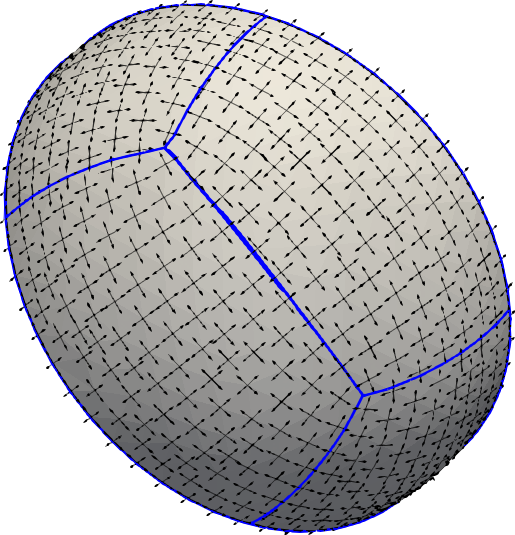
\includegraphics[scale=0.38]{images/align.png}
\caption{Alignement du champ de croix.}
\label{align}
\end{figure}

\begin{figure}[!h]
\centering
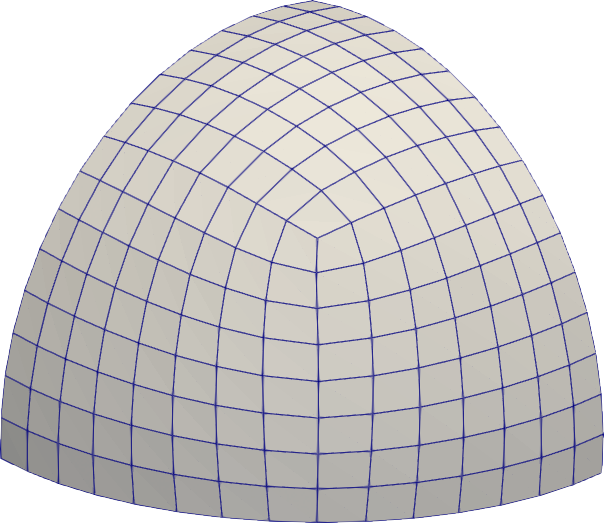
\includegraphics[scale=0.35]{images/huit_quad.png}\hfill
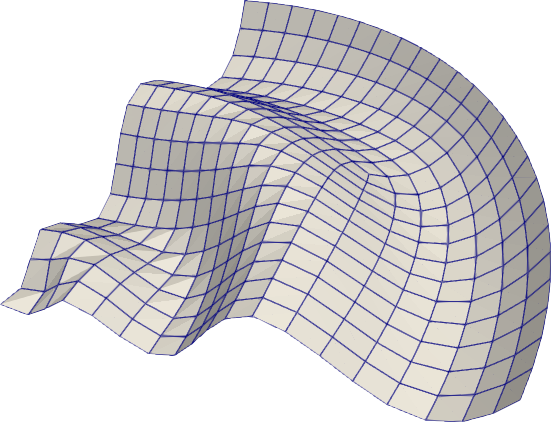
\includegraphics[scale=0.4]{images/vagues.png}
\caption{Autres illustrations de maillage quadrilatéral de surfaces courbes dans l'espace.}
\label{another}
\end{figure}


\section{Analyse de convergence}

Dans cette section, de manière similaire à l'étude exposée dans la section précédente, nous nous posons la question de savoir si le maillage quadrilatéral obtenu par la méthode précédemment décrite est bien un maillage du domaine de départ $\Omega$. Pour répondre à cette question, il suffit de montrer que le partitionnement construit sur $\Omega_h$, que nous notons $\mathcal{P}_h$, converge vers un partitionnement de $\Omega$ comprenant des partitions quadrilatérales.

Notons cependant que le lift à considérer ici est un lift surfacique et dépend de toute la surface. Plus précisément, si $\eta$ est une fonction définie sur $\Omega$ et $\eta_h$ sa représentation élément fini définie sur $\Omega_h$, alors le lift de $\eta_h$ de $\Omega_h$ vers $\Omega$ est donné par :
\begin{equation}
\eta_h(p)=[\mathbf{L}_{\Omega_h}^{\Omega}\eta_h](p-d(p)N(p))\text{ pour tout }p\in\Omega_h,
\end{equation}
où $N(p)$ est la normale sortante en $p$. Nous supposons que $\Omega$ est représenté globalement par une fonction de distance orientée $d$ définie sur un sous-ensemble ouvert $U$ de $\mathbb{R}^2$ tel que
\[
\Omega=\{x\in U,~d(x)=0\},
\]
avec $d$ appartenant à $\mathcal{C}^{k,\alpha}(U)$, $\nabla d\neq 0$ ($k\in\mathbb{N}\cup\{0\}$, $0\leq\alpha\leq 1$). Il résulte des travaux de \cite{dziuk1988finite} que $[\mathbf{L}_{\Omega_h}^{\Omega}\eta_h]$ converge vers $\eta$, et que l'erreur de représentation de la géométrie est d'ordre $2$, là où l'erreur d'approximation du schéma numérique est d'ordre $1$.

La suite de l'analyse est analogue à ce qui a été fait dans la sous-section \ref{subsec:analyse_convergence}. Plus précisément, en adoptant les mêmes notations, on retrouve la même inégalité entre la ligne de champ du champ $\bar{v}$ d'origine $p$ et de vecteur initial $w$ (notée $I(p,w,\bar{v})$) et l'approximation d'une ligne de champ du champ $\bar{v}_h$ de même origine avec le même vecteur initial (notée $I_h(p,w,\bar{v}_h)$):
\begin{eqnarray*}
||I(p,w,\bar{v})-I_h(p,w,\bar{v}_h)||&\leq& ||I(p,w,\bar{v}_h)-I_h(p,w,\bar{v}_h)|| +\\\\
&&||I(p,w,[\mathbf{L}_{\Omega_h}^{\Omega}\bar{v}_h])-I(p,w,\bar{v}_h)||+\\\\
&&||I(p,w,\bar{v})-I(p,w,[\mathbf{L}_{\Omega_h}^{\Omega}\bar{v}_h])||.
\end{eqnarray*}
On a:
$$||I(p,w,\bar{v})-I_h(p,w,\bar{v}_h)||\xrightarrow[h \to 0]{} 0,$$
puisque chaque terme converge vers $0$. Ainsi, on déduit que les séparatrices internes construites sur $\Omega_h$ convergent vers les séparatrices internes construites sur $\Omega$ et, puisque $\Omega_h$ converge vers $\Omega$, on a la convergence des séparatrices de bord.


\section{Génération de champs de croix}


Nous présentons ici les différents méthodes utilisées dans ce chapitre pour la génération de champs de croix  initiaux qui sont le point d'entrée de notre opération d'alignement.

\subsection{L'\'Equation de Laplace}
\label{subsec:laplace_equation_generation_space}

Il s'agit de la version surfacique de la méthode présentée dans la sous-section \ref{subsec:laplace_equation_generation}. L'idée consiste à résoudre l'équation:

\begin{equation}
\left\{
\begin{array}{lcll}
\Delta f &=& 0 &\mbox{ dans }\Omega,\\\\
f(p)&=&\left(\cos(4\theta_{\bar{n}}(p)), \sin(4\theta_{\bar{n}}(p))\right) & \mbox{ sur } \partial\Omega,
\end{array}
\right.
%\label{eqn:frey_vectoriel}
\end{equation}

Le champ de croix $\bar{u}$ est ensuite donné pour tout $p\in\Omega$ par:
$$
\bar{u}(p)=
\left\{
\begin{array}{ll}
\mathbf{R}(\theta_f/4)X_p& \mbox{ si }f\neq 0,\\\\
0&\mbox{ sinon}.
\end{array}
\right.
$$
où $X_p$ est la référence arbitraire choisie dans l'espace tangent en $p$. Cette équation peut être résolue sur $\Omega_h$ par la méthode des éléments finis.
\begin{figure}[!h]
\centering
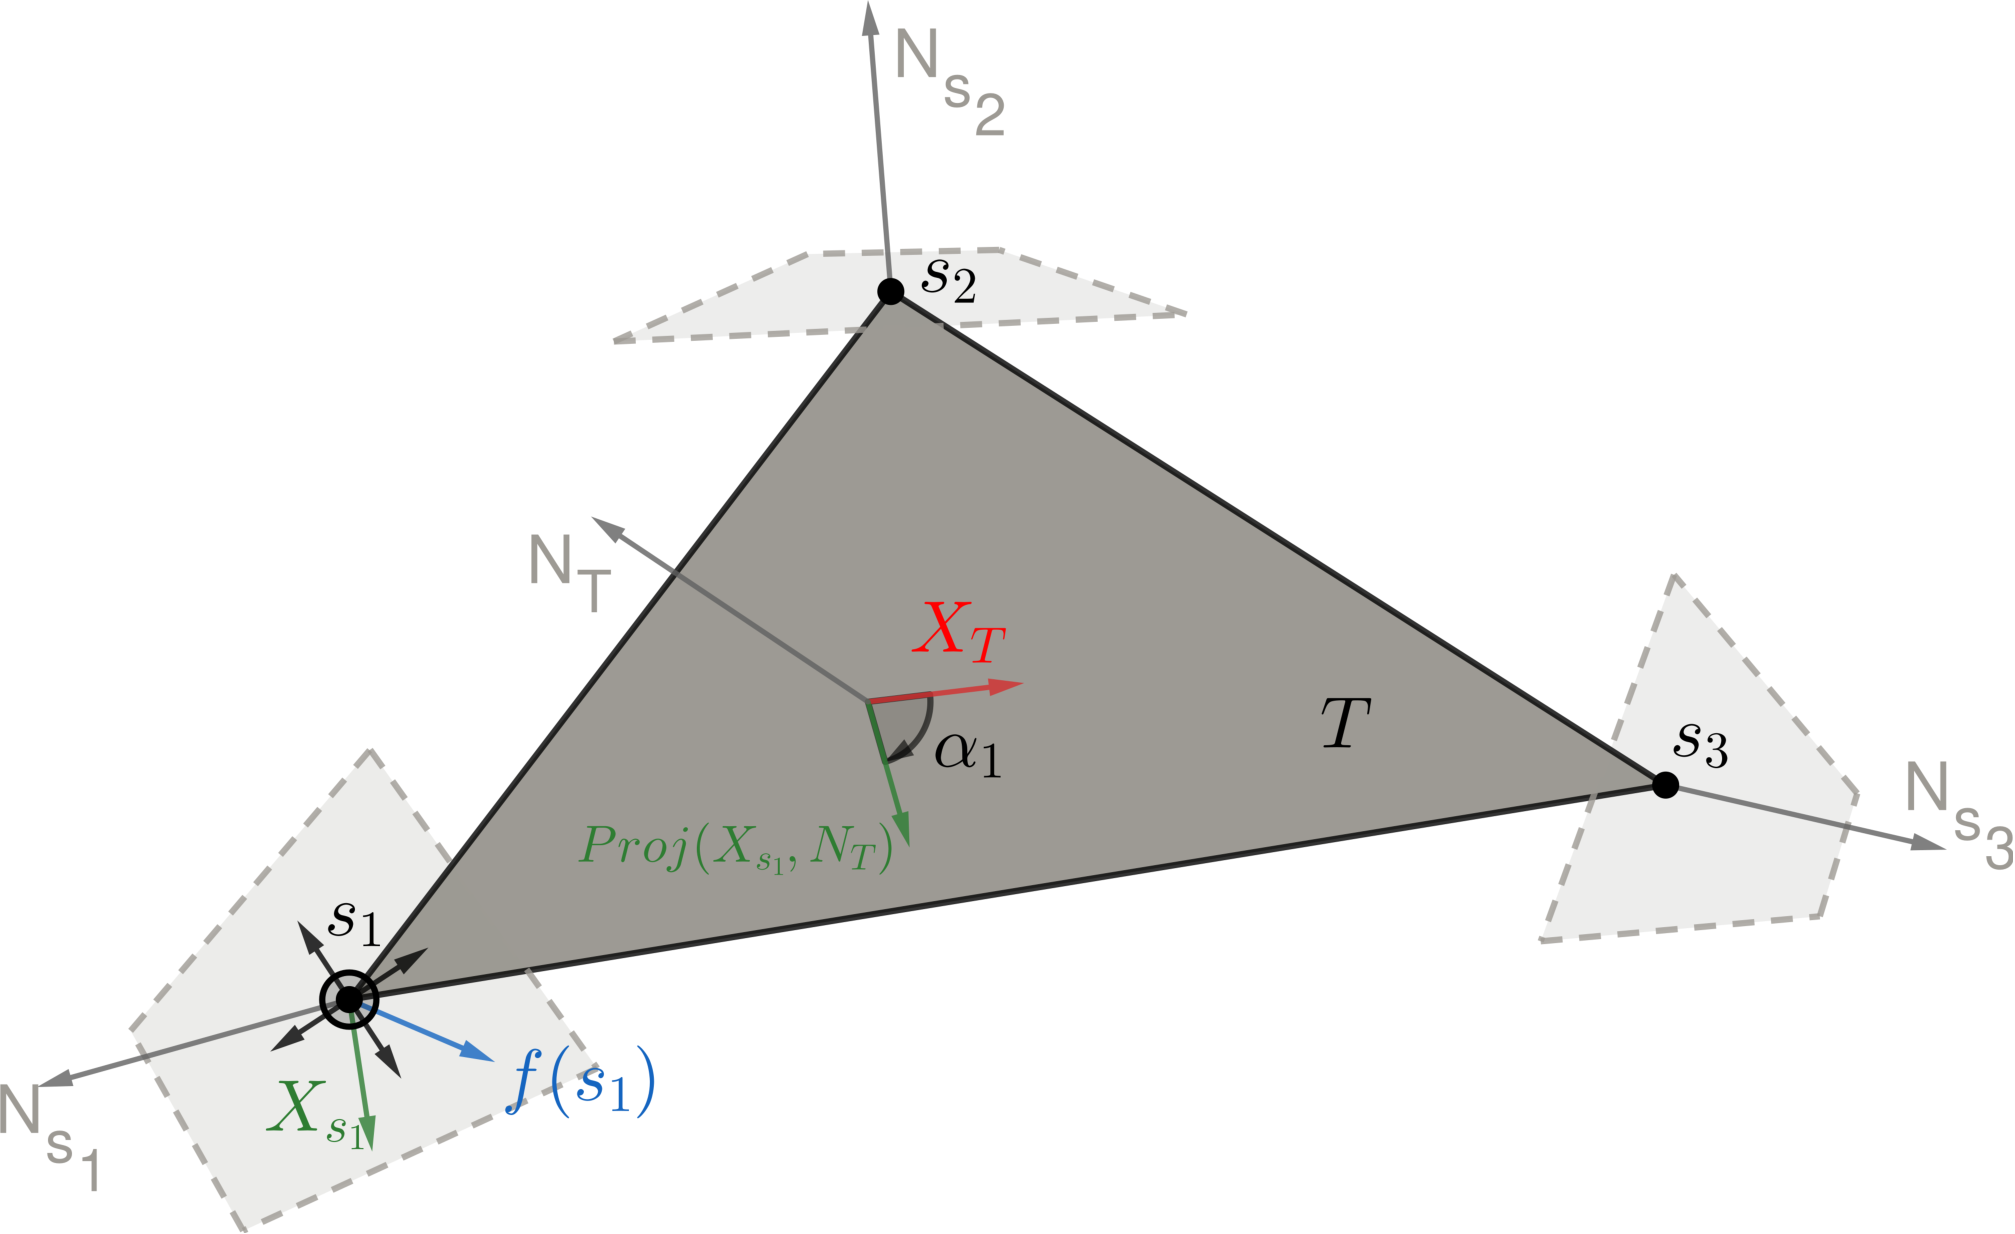
\includegraphics[scale=0.45]{images/triangle_space_laplace.pdf}
\caption{Alignement du champ de croix.}
\label{triangle_space_laplace}
\end{figure}
Étant donné un triangle $T$ de sommets $s_i$, $i\in\llbracket1, 3\rrbracket$, désignons par $\alpha_i$ l'angle entre la projection sur le triangle $T$ de la référence $X_{s_i}$ de l'espace tangent en $s_i$ et la référence choisi dans l'espace tangent associé à $T$ noté $X_T$. La matrice de rigidité élémentaire est alors donnée par:
$$
\mathbf{P}^{-1}\mathbf{K}\mathbf{P},
$$
où $\mathbf{P}$ est donné par:
$$
\mathbf{P}=
\begin{pmatrix}
\cos(4\alpha_1) & 0 & 0 & \sin(4\alpha_1) & 0 & 0 \\
0 & \cos(4\alpha_2) & 0 & 0 & \sin(4\alpha_2) & 0 \\
0 & 0 & \cos(4\alpha_3) & 0 & 0 & \sin(4\alpha_3) \\
-\sin(4\alpha_1) & 0 & 0 & \cos(4\alpha_1) & 0 & 0 \\
0 & -\sin(4\alpha_2) & 0 & 0 & \cos(4\alpha_2) & 0 \\
0 & 0 & -\sin(4\alpha_3) & 0 & 0 & \cos(4\alpha_3) \\
\end{pmatrix}
$$
et $\mathbf{K}$ est donné par:
$$
\mathbf{K}=
\begin{pmatrix}
\mathbf{k} & 0 \\
0 & \mathbf{k} \\
\end{pmatrix},
$$
avec $\mathbf{k}$ la matrice de rigidité élémentaire dans le cas scalaire que l'on calcule avec la formule cotangente du Laplacien présentée dans l'annexe \ref{Op_lap_discr}.



\subsection{Connexions triviales}

Dans \cite{crane2010trivial}, les auteurs présentent un algorithme simple pour construire des connexions sur des surfaces discrètes qui sont aussi lisses que possible partout, sauf sur un ensemble de singularités isolées avec un indice donné. Ces connexions sont résolues en résolvant un seul système linéaire construit à partir d'opérateurs standards. Nous exposons ici cet algorithme pour un domaine simplement connexe où les singularités sont spécifiées par rapport aux triangles.

Soit $\Omega_h$ un maillage triangulaire. Nous souhaitons construire un champ de croix $\bar{u}_h$ sur $\Omega_h$. Pour ce faire, nous cherchons à résoudre un ensemble d'angles d'ajustement qui indique comment faire pivoter un vecteur chaque fois qu'il se déplace le long d'une arête. Soit $\alpha$ ce champ d'angle d'ajustement et notons $\alpha_{ij}$ l'angle d'ajustement associé à l'arête $s_is_j$ de sommets $s_i$ et $s_j$. Remarquons que $\alpha$ est donc un vecteur de réels dont la taille est égale au nombre d'arêtes. Nous attribuons une orientation arbitraire à chaque arête, puis orientons chaque triangle dans le sens positif de la normale au triangle. Nous construisons ensuite une matrice $A$ représentant les interactions entre les triangles et les arêtes du maillage. Il s'agit donc d'une matrice rectangulaire ayant comme nombre de lignes le nombre de triangles et comme nombre de colonnes le nombre d'arêtes, définie par :

$$A_{ij} =
\begin{cases}
1 & \text{si l'arête } i \text{ est contenue dans le triangle } j \text{ avec la même orientation}, \\\\
-1 & \text{si l'arête } i \text{ est contenue dans le triangle } j \text{ avec l'orientation contraire}, \\\\
0 & \text{sinon}.
\end{cases}
$$
pour contrôler le placement des singularités, nous spécifions pour chaque triangle l'indice $k_i$ désiré, puis nous assemblons le vecteur $b$ donné pour chaque triangle $T_i$ par :
$$
b_i = 2k_i\pi-K_i,
$$
où $K_i$ désigne le défaut d'angle (holonomie) autour du triangle $T_i$ dû à la rotation de la normale surfacique autour du triangle. Enfin, pour calculer les angles d'ajustement, nous résolvons le problème convexe :
\[
\min_\alpha \|\alpha\|_2 \quad \text{tel que} \quad A\alpha = b.
\]
Dans le cas où la matrice $A$ a un rang plein, la méthode des multiplicateurs de Lagrange donne une solution unique. Cette solution est donnée par la formule $\alpha = -A^T (AA^T)^{-1} b$. Dans ce cas, la solution est unique car la contrainte linéaire est suffisamment restrictive pour éliminer toute ambiguïté dans la solution. Une fois que nous avons le vecteur $\alpha$, la construction d'un champ de croix est simple. Nous attribuons une croix arbitraire en un point que nous propageons sur le reste des sommets du maillage. Sur une arête $s_is_j$, pour trouver la croix au sommet $s_j$ étant donné la croix en un sommet $s_i$, nous avons :
$$
\bar{u}_h(s_j)=
\begin{cases}
\{\mathbf{R}(\beta_j+m\pi/2)X_{s_j},\quad m\in\llbracket0, 3\rrbracket\}\\\\
\beta_j = \beta_i - \theta_{ij} + \theta_{ji} - \alpha_{ij},
\end{cases}
$$
où $\beta_k$ est l'angle par rapport à la référence $X_{s_k}$ défini au sommet $s_k$, et $\alpha_{ij}$ est l'angle d'ajustement de l'arête $s_is_j$. Enfin, $\theta_{ij}$ et $\theta_{ji}$ sont respectivement les angles entre l'arête $s_is_j$ et les références fixées aux sommets $s_i$ et $s_j$. Les champs de croix illustrés sur les figures \ref{fig:separatrice_illustration_surface} et \ref{nonalign} ont été généré avec cette approche.


%somme de champs de croix\\
%connexion\\
%Dans \cite{crane2010trivial, de2010trivial} les auteurs proposent un algorithme pour calculer des connexions triviales avec des singularités prescrites sur des surfaces discrètes générales. Nous adaptons cet algorithme pour construire des champs de croix défini sur les sommets d'un maillage triangulaire.
